
\documentclass{article} % For LaTeX2e
\usepackage{iclr2027_conference,times}

% Optional math commands from https://github.com/goodfeli/dlbook_notation.
\input{math_commands.tex}

\usepackage{algorithm}
\usepackage{algpseudocode}
\usepackage{hyperref}
\usepackage{cleveref}
\usepackage{url}
\usepackage{svg}
\usepackage{booktabs}
\usepackage{longtable}
\usepackage{etoolbox}
\usepackage{graphicx}
\usepackage[table,dvipsnames]{xcolor}
\usepackage{nicematrix}
\usepackage{multirow}
\usepackage{makecell}
\usepackage{placeins}
\usepackage{xspace}
% Keep floats compact while giving LaTeX enough flexibility to avoid
% prematurely ending a page when several figures or tables are queued.
\setcounter{topnumber}{3}
\setcounter{bottomnumber}{2}
\setcounter{totalnumber}{5}
\renewcommand{\bottomfraction}{0.80}
\renewcommand{\floatpagefraction}{0.75}
\setlength{\textfloatsep}{11pt plus 2pt minus 2pt}
\setlength{\floatsep}{9pt plus 2pt minus 2pt}
\setlength{\intextsep}{11pt plus 2pt minus 2pt}
\setlength{\abovecaptionskip}{9pt}
\setlength{\belowcaptionskip}{0pt}
\hbadness=10000
\vbadness=10000
\ifdefined\pdfsuppresswarningpagegroup
  \pdfsuppresswarningpagegroup=1
\fi
\makeatletter
\@ifpackagelater{longtable}{2025/12/22}{}{%
  \patchcmd{\LT@output}
    {\copy\LT@foot\vss}
    {\copy\LT@foot\vskip\z@\@plus1fil\@minus\normalbaselineskip}
    {}{}%
  \patchcmd{\LT@output}
    {\copy\LT@foot\vss}
    {\copy\LT@foot\vskip\z@\@plus1fil\@minus\normalbaselineskip}
    {}{}%
}
\makeatother
\newcommand{\collaborativelearning}{{\fontfamily{lmtt}\selectfont\textbf{Collaborative Learning}}\xspace}
\newcommand{\lmttbf}[1]{{\fontfamily{lmtt}\selectfont\bfseries #1}}

\title{Reallocating Reasoning across Models\\ via Learned Collaboration}

\author{Antiquus S.~Hippocampus, Natalia Cerebro \& Amelie P. Amygdale \thanks{ Use footnote for providing further information
about author (webpage, alternative address)---\emph{not} for acknowledging
funding agencies.  Funding acknowledgements go at the end of the paper.} \\
Department of Computer Science\\
Cranberry-Lemon University\\
Pittsburgh, PA 15213, USA \\
\texttt{\{hippo,brain,jen\}@cs.cranberry-lemon.edu} \\
\And
Ji Q. Ren \& Yevgeny LeNet \\
Department of Computational Neuroscience \\
University of the Witwatersrand \\
Joburg, South Africa \\
\texttt{\{robot,net\}@wits.ac.za} \\
\AND
Coauthor \\
Affiliation \\
Address \\
\texttt{email}
}

\begin{document}


\maketitle

%\begin{abstract}

%Large language models (LLMs) excel at a wide range of tasks, benefiting from strong knowledge priors, flexible in-context reasoning, and scalable test-time computation. Despite these strengths, single-model reasoning remains vulnerable to error propagation, as later steps continue to depend on the model’s own earlier outputs, leaving reasoning blind spots difficult to independently reassess. To address this limitation, we introduce \textit{model slicing}, which replaces a single large model with multiple smaller, heterogeneous models under a comparable total parameter budget, thereby introducing distinct reasoning perspectives. Building on this idea, we introduce \textit{collaborative learning}, where \textit{pyramid supervision} combines protocol distillation with step-level supervision to train heterogeneous models for effective cross-model collaboration. We evaluate our approach across four task categories: multi-hop question answering, mathematical reasoning, code generation, and open-ended constrained generation. The results show that it improves both task performance and reasoning efficiency, while inducing differentiated collaboration patterns among heterogeneous models. These results show that learned collaboration can transform model heterogeneity into complementary reasoning capabilities. Our code is available at \url{https://anonymous.4open.science/r/collaborativelearning}.

%\end{abstract}

\begin{abstract}

Large language models (LLMs) excel at a wide range of tasks, benefiting from strong knowledge priors, flexible in-context reasoning, and scalable test-time computation. Despite these strengths, single-model reasoning remains vulnerable to error propagation, as later steps depend on the model's own earlier outputs, leaving reasoning blind spots difficult to independently reassess. To address this limitation, we develop \textit{collaborative learning}, encompassing both the construction of heterogeneous collaborators and the learning of effective cross-model collaboration. Specifically, \textit{model slicing} replaces a single large model with multiple smaller, heterogeneous models under a comparable total parameter budget, enabling prior reasoning to be reassessed across distinct model parameterizations. \textit{Pyramid supervision} further combines protocol distillation with step-level supervision to progressively refine reasoning and interaction decisions throughout collaboration. We evaluate our approach across four task categories: multi-hop question answering, mathematical reasoning, code generation, and open-ended constrained generation. The trained heterogeneous models achieve comparable or better task performance and reasoning efficiency than the original large model and established multi-agent system and multi-agent reinforcement learning baselines, while exhibiting differentiated collaboration patterns across tasks. These findings show that learned collaboration turns model heterogeneity into complementary reasoning capabilities. Code is available at \url{https://anonymous.4open.science/r/collaborativelearning} for anonymous review.

\end{abstract}

\section{Introduction}

Large language models (LLMs) have demonstrated capabilities across tasks~\citep{wang2024mmlupro}. Advances highlight the benefits of scaling test-time computation~\citep{snell2025scaling,muennighoff2025s1,wu2025inferencescaling}. Many approaches seek to improve task performance by allowing a single model to structure its reasoning process~\citep{besta2024graphthoughts} and generate, inspect, and revise intermediate steps~\citep{zhou2024selfdiscover,zhang2024restmcts,kumar2025selfcorrect}. However, when the same model both generates and evaluates a solution, it may exhibit self-bias, favoring its own outputs and limiting its ability to identify and correct reasoning errors~\citep{huang2024selfcorrect,xu2024selfbias}. Consequently, errors in intermediate steps may remain undetected and influence subsequent reasoning~\citep{zheng2025processbench}. This motivates \textit{reasoning-state isolation} across models, allowing prior reasoning to be independently reassessed under distinct model parameterizations rather than repeatedly evaluated within the same model's reasoning space~\citep{du2024debate,liang2024mad}.

Accordingly, we develop a \textit{collaborative learning} framework for reasoning and learning across heterogeneous models, as illustrated in Figure~\ref{fig:model_slicing_concept}. Model slicing replaces a single large model with several smaller, heterogeneous models under a comparable total parameter budget~\citep{liu2026collaboration}. Through explicit handoffs of task state between models~\citep{chen2024agentverse}, prior reasoning can be independently reassessed under distinct model parameterizations, thereby enabling model-specific reasoning-state isolation while producing interaction trajectories that capture reasoning and interaction decisions. Together, this isolation and the resulting trajectories provide the structural basis for training heterogeneous models to leverage complementary capabilities~\citep{wang2025mixture,abdulaal2025balancing,chen2025ioa} when questioning, extending, or revising prior conclusions.

\begin{figure}[!t]
\centering
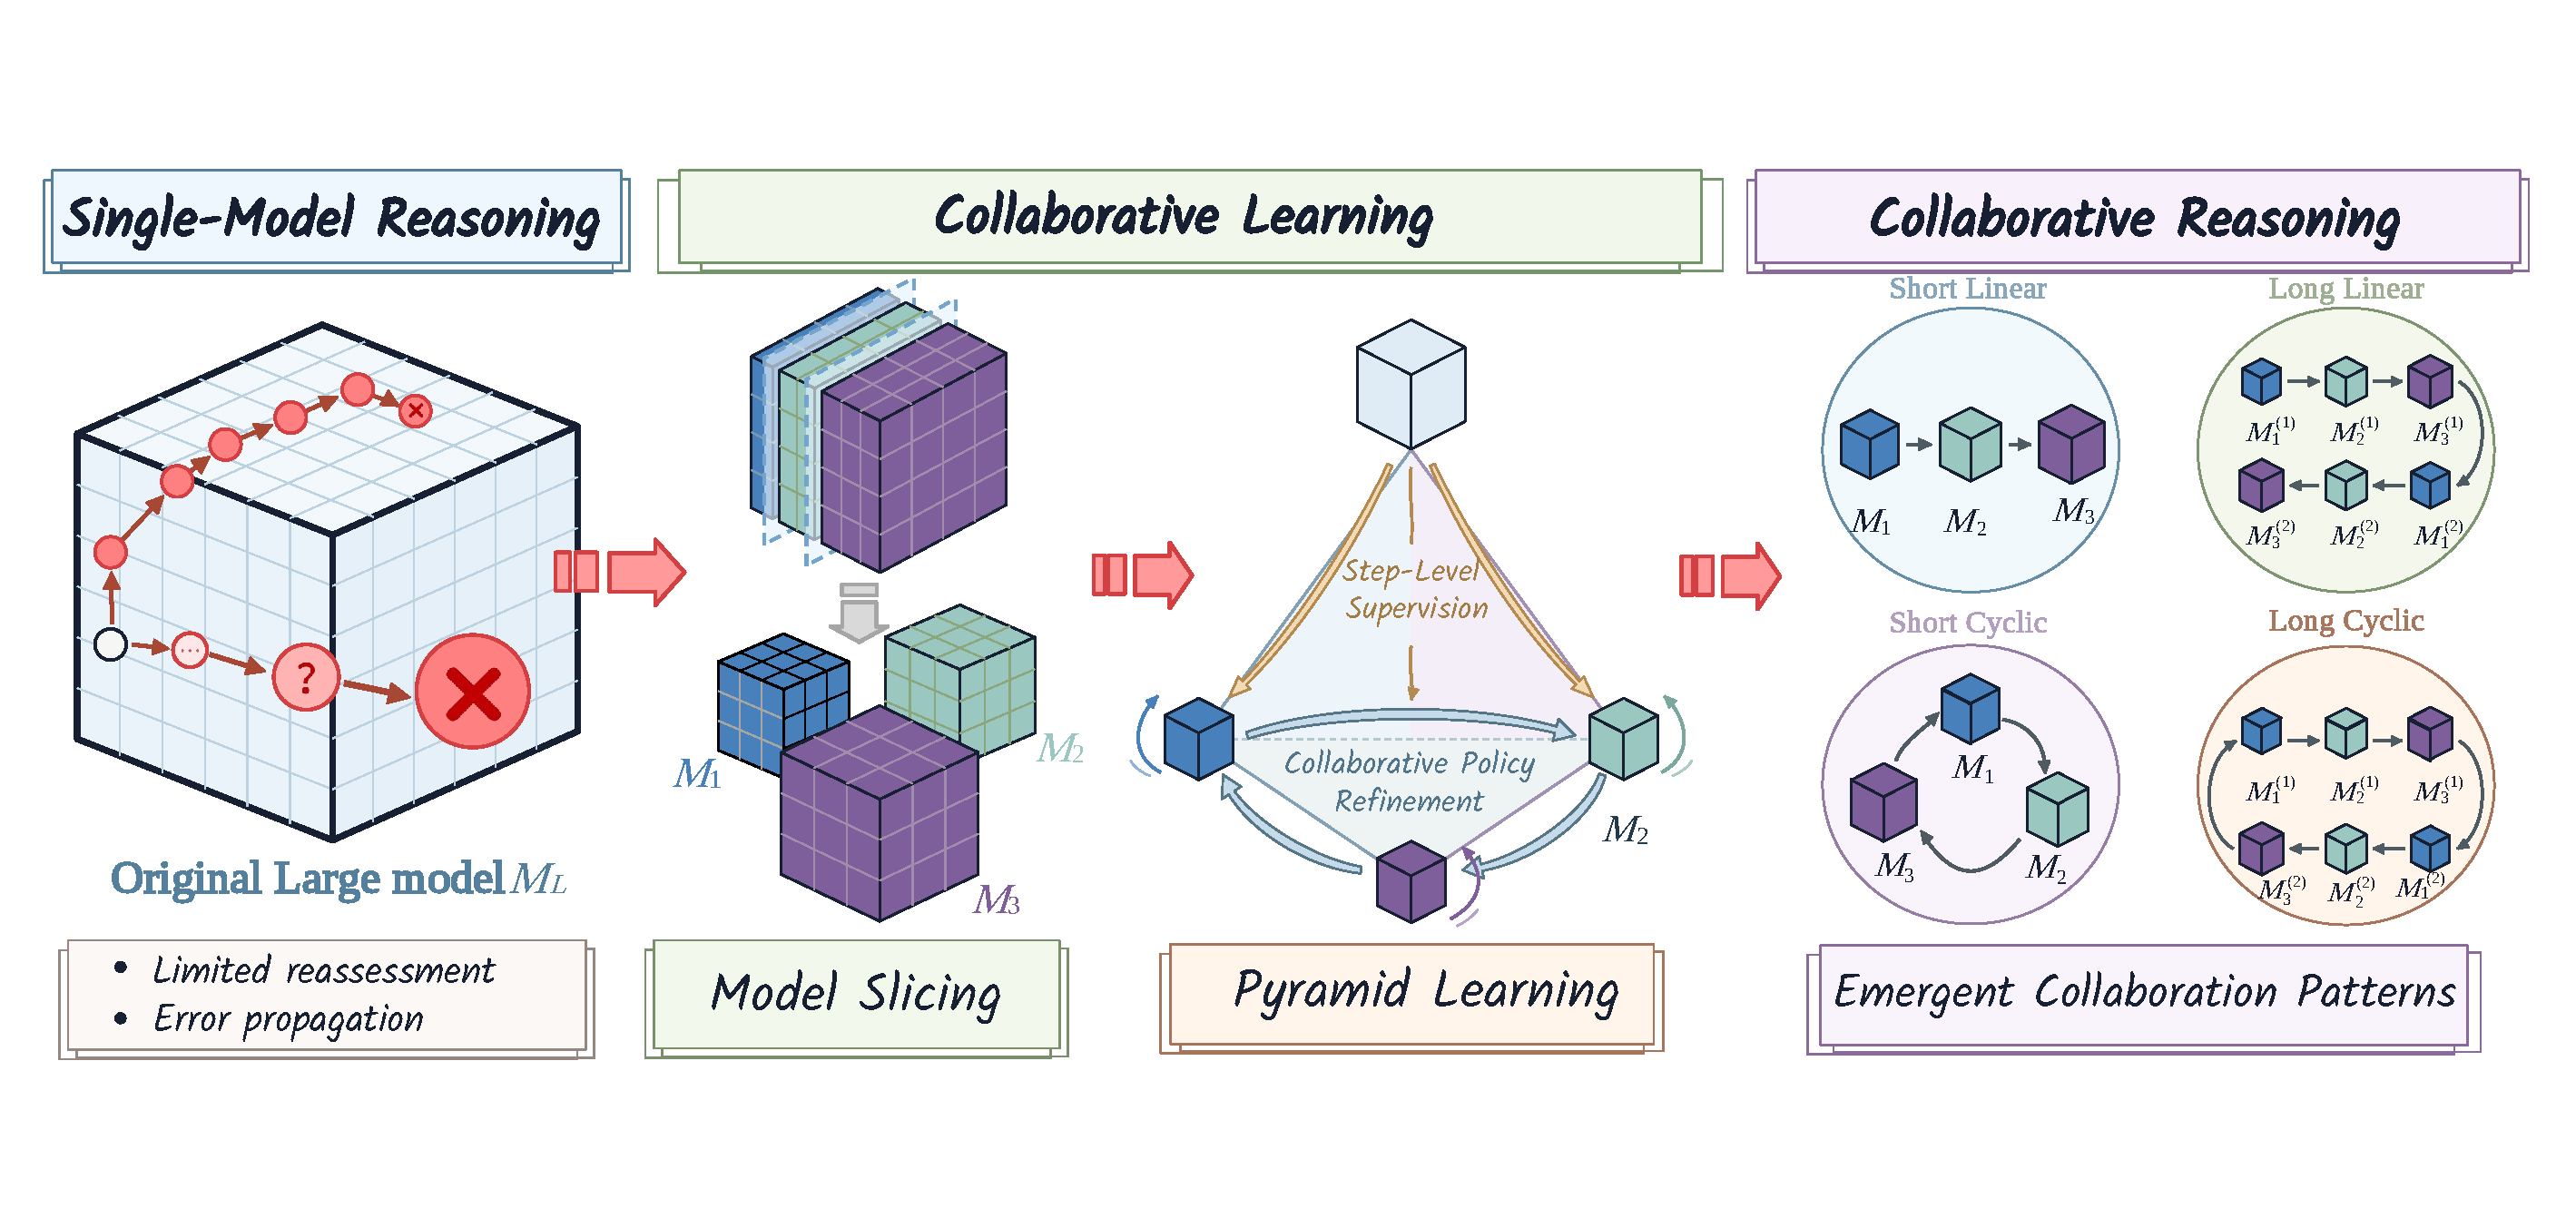
\includegraphics[width=\linewidth]{figures/Figure1.pdf}
\vspace{-1.5em}
\caption{\textbf{Reallocating reasoning across models via learned collaboration.}
Model slicing reallocates a single large model into multiple smaller, heterogeneous models under a comparable parameter budget, enabling reasoning to be reassessed across model parameterizations. Building on this, \textit{collaborative learning} trains heterogeneous models through pyramid supervision that integrates protocol distillation with step-level supervision over complete collaboration trajectories.}
\label{fig:model_slicing_concept}
\end{figure}


Although this structure provides a foundation for cross-model collaboration, outcome-level supervision alone provides insufficient guidance for intermediate reasoning and interaction decisions throughout the collaborative process~\citep{lightman2024verify,wang2024mathshepherd,setlur2025progress}. To address this limitation, we propose \textit{pyramid supervision}, which progressively refines collaboration among heterogeneous models through fine-grained supervision. It incorporates supervision over intermediate reasoning and interaction decisions along model-generated collaboration trajectories, while integrating task-level rewards to jointly optimize local decision quality and overall task performance~\citep{zhuge2025agentjudge}. Through this training mechanism, heterogeneous models learn effective collaborative reasoning and develop differentiated interaction patterns across tasks.

We evaluate our approach across four task categories: multi-hop question answering, mathematical reasoning, code generation, and open-ended constrained generation. With a total parameter budget comparable to that of the original large model, the trained heterogeneous models collectively match or outperform the original model as well as established multi-agent system (MAS) and multi-agent reinforcement learning (MARL) baselines. Analysis of interaction trajectories further reveals reduced reasoning redundancy and differentiated collaboration patterns characterized by questioning, complementing, and revising prior reasoning. Together, these results suggest that collaborative reasoning across heterogeneous models can improve task performance while enabling complementary contributions and the reassessment of prior reasoning across distinct model parameterizations.


Our key contributions are summarized in three points:

\begingroup
\setlength{\leftmargini}{1em}
\begin{itemize}

\item We propose a trainable paradigm for collaborative reasoning and learning across heterogeneous models, enabling prior reasoning to be independently reassessed across distinct model parameterizations while progressively learning cross-model collaboration from interaction trajectories.

\item We introduce model slicing and pyramid supervision. Model slicing replaces a large model with heterogeneous models under a comparable budget and enables reasoning-state isolation through task-state handoffs. Pyramid supervision refines model-generated collaboration through fine-grained supervision over reasoning and interaction decisions with task-level rewards.

\item We validate collaborative learning across four reasoning task categories. Compared with the original large model, established MAS baselines, and MARL methods, the trained heterogeneous models achieve comparable or better task performance and reasoning efficiency, while exhibiting emergent task-adaptive cross-model collaboration patterns through training.

\end{itemize}
\endgroup

\section{Method}

\begin{figure}[!t]
\centering
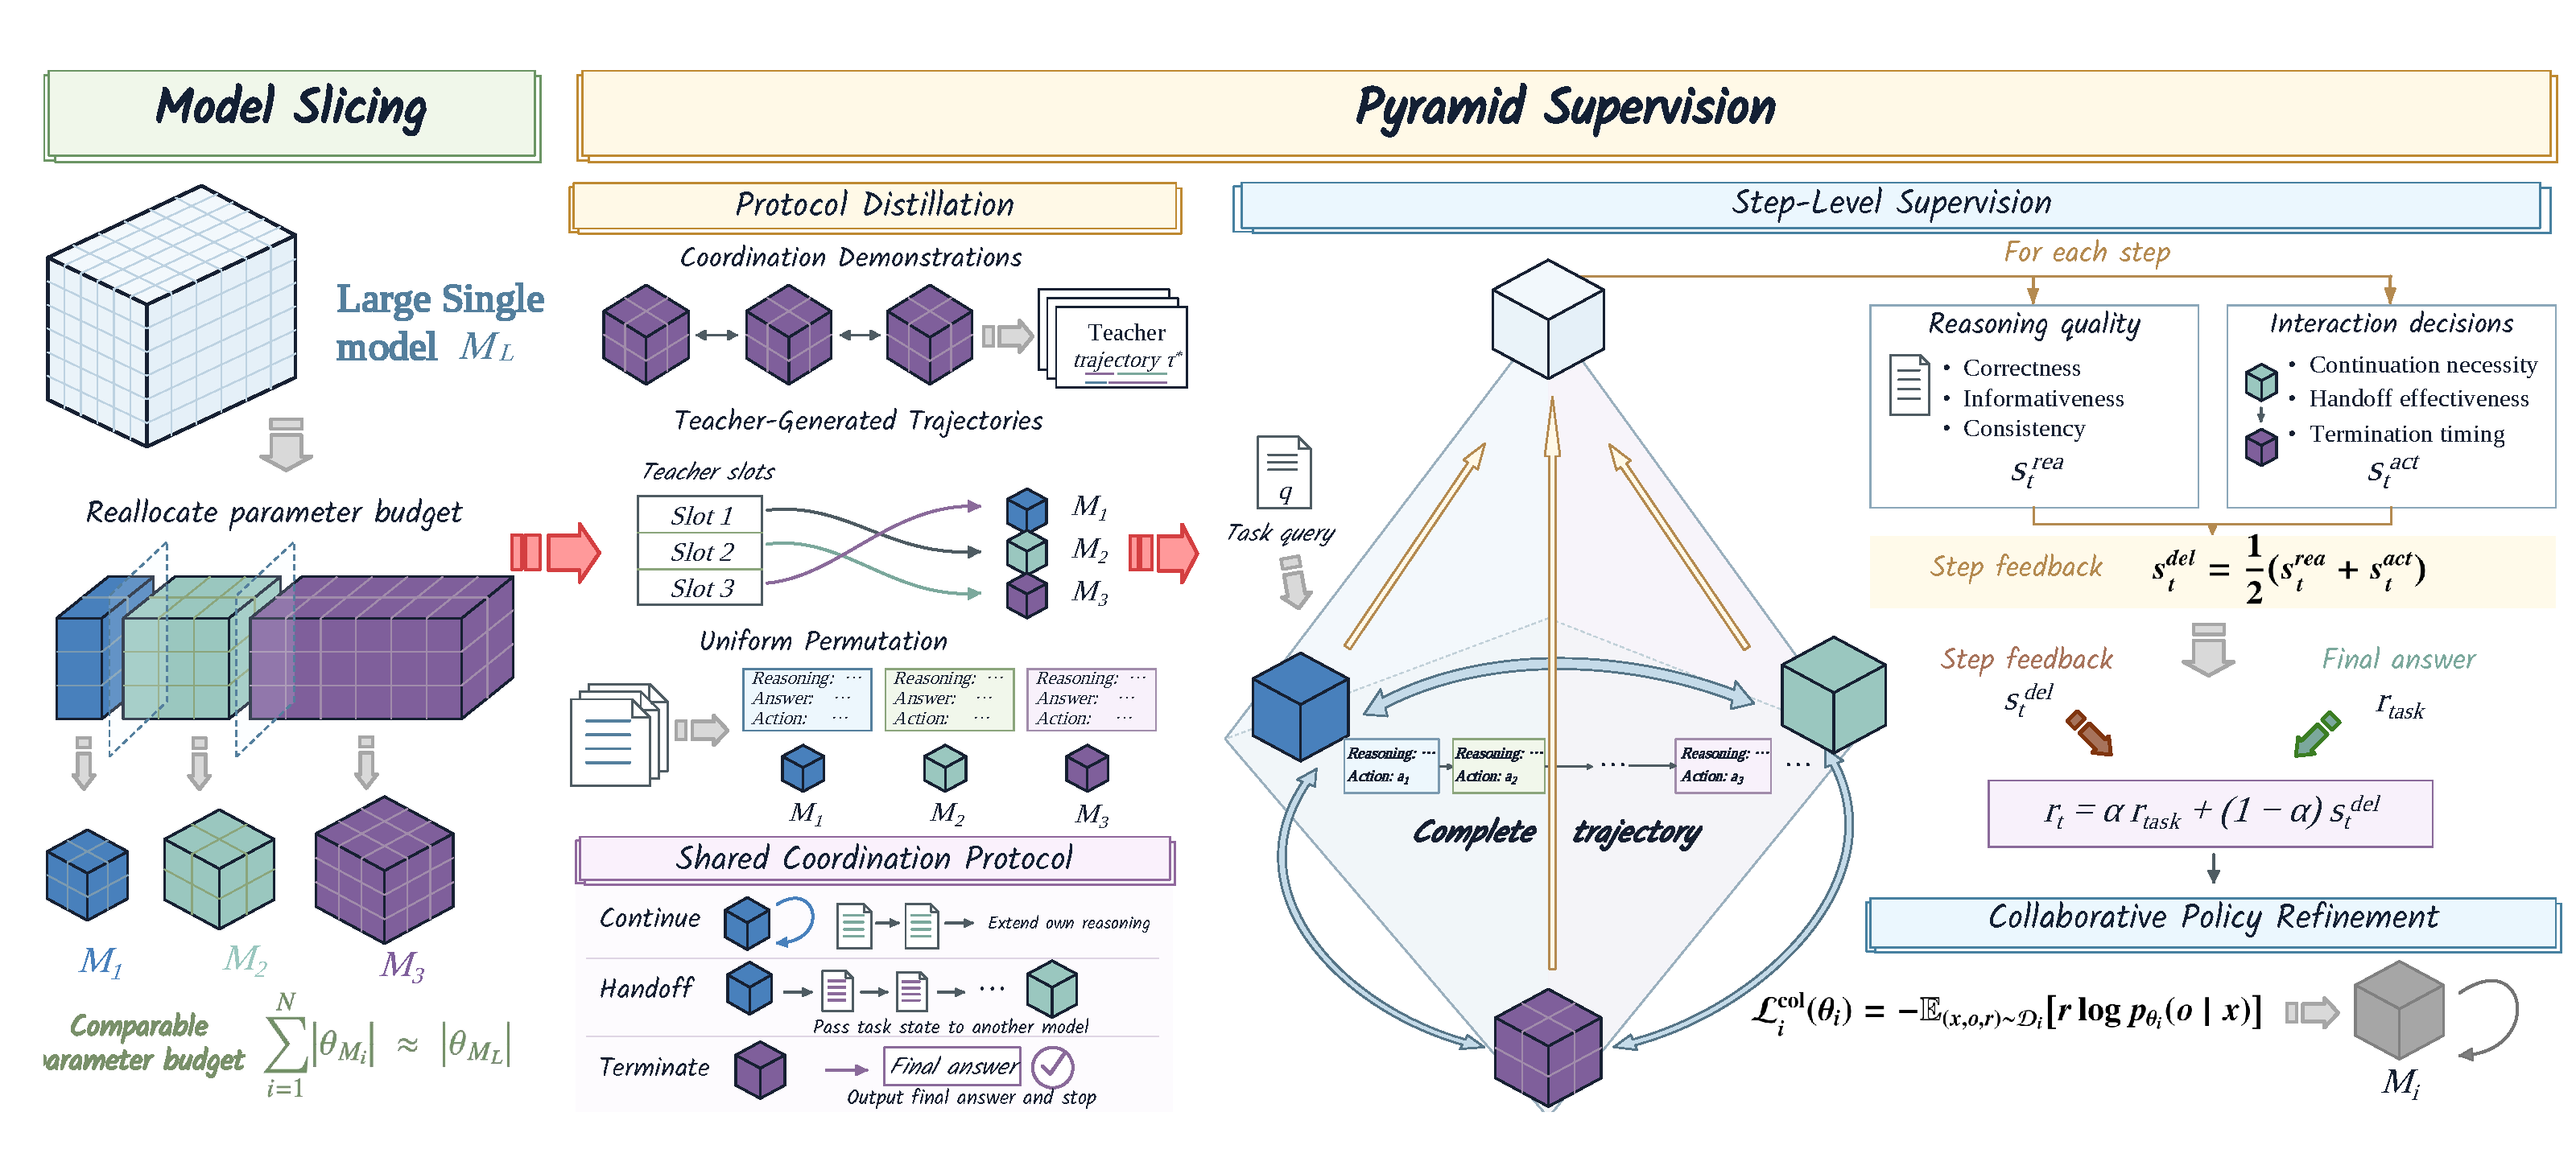
\includegraphics[width=\linewidth]{figures/Figure2.pdf}
\vspace{-1.25em}
\caption{\textbf{Overview of collaborative learning.} (a) Model slicing constructs smaller, heterogeneous models under a comparable total parameter budget. (b) Pyramid supervision initializes collaboration through protocol distillation and refines it through step-level supervision. The original large model evaluates each step’s reasoning and interaction decisions within the complete trajectory. Step-level scores and final task rewards jointly guide collaborative policy refinement.}
\label{fig:framework}
\end{figure}

%Collaborative reasoning is formulated as an iterative process among heterogeneous models. The models share context through a unified interaction protocol and hand off the task state across models, allowing the receiving model to continue reasoning with its own parameters and perform operations such as questioning, extending, or revising prior conclusions across distinct model parameterizations ($\triangleright$ \Cref{sec:collaborative_reasoning}). Building on this process, collaborative learning trains effective cross-model collaboration through model slicing and pyramid supervision, with the overall pipeline illustrated in Figure~\ref{fig:framework} ($\triangleright$ \Cref{sec:collaborative_learning}).

Collaborative reasoning characterizes an iterative reasoning process among heterogeneous models, where explicit task-state handoffs under a unified interaction protocol allow prior reasoning to be continually reassessed by models with different parameters ($\triangleright$ \Cref{sec:collaborative_reasoning}). To realize this process, collaborative learning constructs a heterogeneous model set through model slicing and learns effective cross-model collaboration through pyramid supervision ($\triangleright$ \Cref{sec:collaborative_learning}).




\subsection{Collaborative Reasoning}

\label{sec:collaborative_reasoning}

Collaborative reasoning refers to a process in which multiple models jointly construct a solution through successive contributions~\citep{yin2023exchange,chen2024reconcile}. We define a unified interaction protocol that specifies how heterogeneous models generate reasoning and retain, transfer, or terminate control\footnote{Response fields and action-specific output requirements are detailed in Appendix~\ref{app:protocol}.}. For a task input $q$, each interaction step $t$ is represented by

\vspace{-1em}

\begin{equation}
z_t = (i_t, x_t, y_t, a_t)
\end{equation}
where $i_t$ denotes the active model $M_{i_t}$, $x_t$ contains the task input and preceding interaction history, $y_t$ is the current reasoning, and $a_t$ is the interaction action. The action space is defined as
\begin{equation}
a_t \in \{\texttt{continue},\texttt{terminate}\}
\cup {\texttt{handoff}(j) \mid j \in {1,\ldots,N},\ j \neq i_t}
\end{equation}
where \texttt{continue} keeps control with the model, \texttt{handoff(j)} transfers the task state and control to $M_j$, and \texttt{terminate} ends collaborative reasoning. A complete trajectory is represented as
\begin{equation}
\tau = (z_1,z_2,\ldots,z_T)
\end{equation}
where $T$ denotes the total number of interaction steps recorded in the complete trajectory.

Through \texttt{handoff}, different models can use their own parameters to perform operations such as extending, questioning, or revising prior conclusions, allowing reasoning to be reassessed across distinct model parameterizations. The resulting trajectories record both reasoning and interaction decisions and serve as the optimization targets for subsequent collaborative learning.

\subsection{Collaborative Learning}
\label{sec:collaborative_learning}

Collaborative learning encompasses both the construction of heterogeneous collaborators and the learning of cross-model collaboration, with the pipeline illustrated in Figure~\ref{fig:framework}. Model slicing constructs heterogeneous collaborators under a comparable parameter budget, providing the structural basis for cross-model reasoning. Pyramid supervision guides collaborative learning through protocol distillation and step-level supervision, progressively refining models' reasoning and interaction decisions while integrating task-level rewards throughout the collaborative reasoning process.

\subsubsection{Model Slicing}
\label{sec:model_slicing}

Model slicing replaces a single large model with multiple smaller, independently parameterized models under a comparable total parameter budget, constructing a heterogeneous model set for collaborative learning. Let $M_L$ denote the original large model with parameters $\theta_L$. We have
\vspace{-0.3em}
\begin{equation}
\mathcal{M} = {M_1, \ldots, M_N},
\qquad \sum_{i=1}^{N} |\theta_i| \approx |\theta_L|
\end{equation}
\vspace{-0.1em}
where $\theta_i$ denotes the parameters of $M_i$, and $|\theta|$ denotes the parameter count.

These models differ in size and parameters and are not obtained by directly partitioning the weights of $M_L$. Together with task-state handoffs, this heterogeneous model set enables model-specific \textit{reasoning-state isolation} across distinct model parameterizations throughout the collaborative reasoning process, providing the structural basis for subsequent collaborative learning.


\subsubsection{Pyramid Supervision}
\label{sec:Pyramid_Supervision}

We introduce \textit{pyramid supervision} to progressively train collaboration within the heterogeneous model pool. It consists of protocol distillation for interaction initialization and step-level supervision for refining model-generated collaboration through fine-grained reasoning and interaction feedback.

\noindent\textbf{Protocol Distillation.}\quad
Although the interaction protocol specifies how models communicate and transfer control, heterogeneous models do not naturally learn to use it effectively as reasoning evolves. In particular, they must learn when to retain control, hand off the task state, or terminate based on the evolving reasoning context~\citep{zeng2024agenttuning}. We therefore use protocol distillation to initialize cross-model interaction from teacher-generated trajectories~\citep{chen2024magdi}.

We select the largest model in $\mathcal{M}$ by parameter count as the teacher $M^\star$ and instantiate $N$ homogeneous copies to form the teacher system:
\begin{equation}
    \mathcal{M}_{\mathrm{teacher}}
    =
    \{M_1^\star,\ldots,M_N^\star\},
    \qquad
    M_j^\star \equiv M^\star,\quad j=1,\ldots,N
\end{equation}

Following the same interaction protocol as the target models, the teacher system generates multi-step trajectories for distillation inputs
$\mathcal{Q}_{\mathrm{distill}}=\{q^{(m)}\}_{m=1}^{K}$:
\begin{equation}
    \tau^{(m)}
    \sim
    P_{\mathcal{M}_{\mathrm{teacher}}}
    \left(\tau \mid q^{(m)}\right),
    \qquad
    m=1,\ldots,K
\end{equation}
We retain qualified trajectories as demonstrations for subsequent distillation.

To avoid a fixed correspondence between teacher slots and target models, we sample a uniform permutation for each trajectory:
\begin{equation}
    \pi^{(m)}
    \sim
    \mathrm{Uniform}(S_N),
    \qquad
    \widetilde{i}_t^{(m)}
    =
    \pi^{(m)}
    \left(i_t^{(m)}\right),
    \quad
    t=1,\ldots,T_m
\end{equation}
where $S_N$ denotes the set of permutations over $\{1,\ldots,N\}$. Within each trajectory, the same permutation is applied consistently to all occurrences associated with each teacher slot, including model indices, handoff targets, and corresponding references in the interaction history. This operation changes only the correspondence between teacher slots and target models across trajectories, while preserving the reasoning content, step order, and handoff structure of the original trajectory.

Let $\widetilde{x}_t^{(m)}$ and $\widetilde{o}_t^{(m)}$ denote the reassigned context and response. Supervision covers the complete response, including reasoning and interaction decisions~\citep{chen2023fireact}. For each model $M_i$, the resulting examples form $\mathcal{D}_i^{\mathrm{pro}}$. Following sequence-level knowledge distillation~\citep{kim2016sequence}, each model minimizes
\begin{equation}
    \mathcal{L}_i^{\mathrm{pro}}
    =
    -\mathbb{E}_{(x,o)\sim\mathcal{D}_i^{\mathrm{pro}}}
    \left[
        \log p_{\theta_i}(o\mid x)
    \right]
\end{equation}

This objective initializes cross-model interaction capabilities in the heterogeneous models, providing a stable starting point for trajectory-level refinement of reasoning and interaction decisions.

\noindent\textbf{Step-Level Supervision.}\quad
After protocol distillation, the heterogeneous models perform collaborative reasoning under the shared interaction protocol, generating trajectories for subsequent optimization. For a given training task $q$, a collaborative trajectory is sampled as
\begin{equation}
    \tau
    =
    (z_1,\ldots,z_T)
    \sim
    P_{\mathcal{M}}(\tau\mid q)
\end{equation}
where $P_{\mathcal{M}}$ is induced by the current models and the shared interaction protocol.

Learning effective collaboration from these trajectories requires identifying the contribution of each reasoning and interaction decision to the overall process~\citep{foerster2018coma}. The value of an individual step depends not only on its local correctness but also on how it influences subsequent collaboration. We therefore retain the original large model $M_L$ as an evaluator $\mathcal{J}$, which assesses each step in the context of the complete trajectory~\citep{zhuge2025agentjudge}. Given the task $q$ and trajectory $\tau$, the evaluator produces two complementary scores:
\begin{equation}
    \left\{
    \left(
    s_t^{\mathrm{rea}},
    s_t^{\mathrm{act}}
    \right)
    \right\}_{t=1}^{T}
    =
    \mathcal{J}(q,\tau),
    \qquad
    s_t^{\mathrm{rea}},s_t^{\mathrm{act}}\in[-1,1]
\end{equation}

The reasoning score $s_t^{\mathrm{rea}}$ evaluates the model's reasoning contribution in terms of correctness, informativeness, and relevance to the task state and interaction history. The interaction score $s_t^{\mathrm{act}}$ evaluates whether its decision to continue, hand off the task state, or terminate appropriately advances the collaborative process. Separating these dimensions avoids conflating reasoning quality with interaction quality. We average the two scores to obtain a step-level score:
\begin{equation}
    s_t^{\mathrm{step}}
    =
    \frac{1}{2}
    \left(
    s_t^{\mathrm{rea}}
    +
    s_t^{\mathrm{act}}
    \right)
\end{equation}
\vspace{-1em}

\noindent\textit{Reward integration.}\quad
Step-level scores provide fine-grained supervision for intermediate reasoning and interaction decisions, but local decision quality does not necessarily translate into successful task completion. To provide decision-specific feedback while also accounting for the overall task objective, we integrate each step-level score with the final task reward. Let $m(q,\hat{y})\in[0,1]$ denote the task-specific evaluation metric for the final prediction $\hat{y}$. We map it to the same $[-1,1]$ range as the step-level score and define
\begin{equation}
    r_{\mathrm{task}}
    =
    2m(q,\hat{y})-1,
    \qquad
    r_t
    =
    \alpha r_{\mathrm{task}}
    +
    (1-\alpha)s_t^{\mathrm{step}}
    \label{eq:step_reward}
\end{equation}
where $\alpha\in[0,1]$ controls the trade-off between the task-level reward and the step-level score. The resulting reward distinguishes the contributions of intermediate steps across the complete collaborative trajectory while aligning their optimization with the final task objective.

\noindent\textit{Collaborative Policy Refinement.}\quad
Using the combined rewards, we extract the steps at which each model was active from the collaborative trajectories and construct model-specific training data. For model $M_i$, the corresponding training examples are collected as

\begin{equation}
\mathcal{D}_i
=
\left\{
(x_t^{(m)},o_t^{(m)},r_t^{(m)})
\mid
i_t^{(m)}=i
\right\}  
\end{equation}
where $o_t$ denotes the complete response at step $t$, serialized under the shared interaction protocol and including its reasoning, answer, and interaction fields. Following the score-function policy-gradient form, we optimize each model with the reward-weighted objective
\begin{equation}
    \mathcal{L}_i^{\mathrm{col}}(\theta_i)
    =
    -\mathbb{E}_{(x,o,r)\sim\mathcal{D}_i}
    \left[
        r\log p_{\theta_i}(o\mid x)
    \right]
    \label{eq:collaborative_objective}
\end{equation}

This objective increases the likelihood of responses assigned positive rewards and decreases the likelihood of those assigned negative rewards. Because each reward combines step-level evaluation conditioned on the complete trajectory with the final task outcome, each model can adapt its policy according to how its own decisions contribute to the collaborative result, allowing differentiated collaboration patterns to progressively emerge through training~\citep{cui2026prime}.


\section{Experiments}
\label{sec:experiments}

\subsection{Experimental Setup}
\label{sec:experimental_setup}

\noindent\textbf{Datasets.}\quad We use five benchmarks across four task categories: multi-hop question answering (MuSiQue~\citep{trivedi2022musique}), mathematical reasoning (GSM-Hard~\citep{gao2023pal} and MATH~\citep{hendrycks2021math}), code generation (an eight-language MultiPL-E subset~\citep{cassano2023multiple})\footnote{Following the language selection in the Qwen3 technical report~\citep{yang2025qwen3}, we restrict code-generation evaluation to Python, C++, Java, PHP, TypeScript, C\#, Bash, and JavaScript.}, and open-ended constrained generation (Conifer~\citep{sun2024conifer}).

%\noindent\textbf{Baselines.}\quad (1) Single-agent baselines: Qwen3-14B~\citep{yang2025qwen3} and its self-evaluated RL variant (SE-RL)\footnote{SE-RL uses Qwen3-14B to evaluate its own trajectories and provide training feedback for comparison with cross-model feedback. See Appendix~\ref{app:baselines} for training details.}. (2) A homogeneous MAS of three Qwen3-8B models without collaborative learning, testing whether capacity and multi-model inference explain gains. (3) A homogeneous collaborative-learning system (Homo. CL) of three Qwen3-4B models (12B total), trained with the same procedure as our heterogeneous system to isolate the effect of model heterogeneity. (4) Established multi-agent frameworks: MAD~\citep{du2024debate}, AgentVerse~\citep{chen2024agentverse}, AFlow~\citep{zhang2025aflow}, and GPTSwarm~\citep{zhuge2024gptswarm}. (5) MARL methods: MAGRPO~\citep{liu2026collaboration}, MAPoRL~\citep{park2025maporl}, and AT-GRPO~\citep{zhao2026strongermas}.

\noindent\textbf{Baselines.}\quad
(1) Single-agent baselines: Qwen3-14B~\citep{yang2025qwen3} and its self-evaluated RL variant (SE-RL)\footnote{SE-RL uses Qwen3-14B to evaluate its own trajectories and provide training feedback for comparison with cross-model feedback. See Appendix~\ref{app:baselines} for training details.}.
(2) A homogeneous MAS of three Qwen3-8B models (24B total) without collaborative training, serving as a higher-capacity multi-model baseline.
(3) A homogeneous collaborative-learning system (Homo. \lmttbf{CL}) of three Qwen3-4B models (12B total), trained with the same procedure as our heterogeneous system to assess the effect of model heterogeneity in collaborative reasoning.
(4) Established multi-agent frameworks: MAD~\citep{du2024debate}, AgentVerse~\citep{chen2024agentverse}, AFlow~\citep{zhang2025aflow}, and GPTSwarm~\citep{zhuge2024gptswarm}.
(5) MARL methods: MAGRPO~\citep{liu2026collaboration}, MAPoRL~\citep{park2025maporl}, and AT-GRPO~\citep{zhao2026strongermas}.

\noindent\textbf{Metrics.}\quad We report accuracy and F1 on MuSiQue~\citep{trivedi2022musique}, GSM-Hard~\citep{gao2023pal}, and MATH~\citep{hendrycks2021math}. We use weighted pass@1 and macro-language pass@1 for MultiPL-E~\citep{cassano2023multiple}, and Coverage and Explicit for Conifer~\citep{sun2024conifer}\footnote{Definitions and computation details for the Conifer metrics are provided in Appendix~\ref{app:conifer_metrics}.}. Beyond task performance, we analyze handoffs, anomaly rates, reasoning redundancy, and model-wise behavioral distributions to characterize training-induced changes in collaboration patterns.

\noindent\textbf{Implementation Details.}\quad
Model slicing replaces Qwen3-14B ($M_L$)~\citep{yang2025qwen3} with Qwen3-1.7B, Qwen3-4B, and Qwen3-8B (13.7B total), all using the same prompt and action space. Three Qwen3-8B instances generate protocol distillation demonstrations; Qwen3-14B supplies trajectory feedback for pyramid supervision. Experiments run on $8\times$ NVIDIA A800-SXM4-80GB GPUs using model-specific rank-64 LoRA adapters~\citep{hu2022lora} with frozen base parameters\footnote{See Appendix~\ref{app:training} for dataset splits, sample sizes, sampling procedures, and training and inference details, and Appendix~\ref{app:baselines} for baseline implementations.}.

\subsection{Does Our Method Lead to Improved Performance?}
\label{sec:main_results}


\vspace{-1.5em}

\begin{table}[!htbp]
\centering
\vspace{0.4em}
\caption{\textbf{Performance comparison with baseline methods.} Scores are percentages (\%); higher is better. Acc. denotes accuracy; Wtd. and Mac. denote weighted and macro-language pass@1, respectively; Cov. and Expl. denote Coverage and Explicit, respectively. Best and second-best results are shown in \textbf{bold} and \underline{underline}, respectively. $\textcolor[RGB]{241,96,52}{\uparrow}$ and $\textcolor[RGB]{1,179,185}{\downarrow}$ indicate scores above and below the corresponding baseline mean for each metric reported in the table.}
\label{tab:main_results}
\begingroup
\fontsize{12}{14}\selectfont
\setlength{\tabcolsep}{2pt}
\renewcommand{\arraystretch}{1.32}
\setlength{\arrayrulewidth}{0.4pt}
\newcommand{\ResultUp}[1]{\ensuremath{{}_{\textcolor[RGB]{241,96,52}{\scalebox{1.1}{$\scriptstyle\uparrow\!#1$}}}}}
\newcommand{\ResultDown}[1]{\ensuremath{{}_{\textcolor[RGB]{1,179,185}{\scalebox{1.1}{$\scriptstyle\downarrow\!#1$}}}}}
\newcommand{\MainResultsHeaderStrut}{\rule[-0.45em]{0pt}{1.85em}}
\vspace{4pt}
\resizebox{\linewidth}{!}{%
\begin{NiceTabular}{l!{\color{black}\vrule width 0.6pt}*{10}{c}}
\CodeBefore
  \rectanglecolor{CadetBlue!20}{1-1}{2-11}
  \rowcolor{gray!10}{4,6,8,10,12,14}
\Body
\arrayrulecolor{black}
\Xhline{1pt}
\Block[l]{2-1}{\textbf{Method}} & \multicolumn{2}{c}{\MainResultsHeaderStrut\textbf{MuSiQue}} & \multicolumn{2}{c}{\MainResultsHeaderStrut\textbf{GSM-Hard}} & \multicolumn{2}{c}{\MainResultsHeaderStrut\textbf{MATH}} & \multicolumn{2}{c}{\MainResultsHeaderStrut\textbf{MultiPL-E}} & \multicolumn{2}{c}{\MainResultsHeaderStrut\textbf{Conifer}} \\
& {\small\MainResultsHeaderStrut\textbf{Acc.}} & {\small\MainResultsHeaderStrut\textbf{F1}} & {\small\MainResultsHeaderStrut\textbf{Acc.}} & {\small\MainResultsHeaderStrut\textbf{F1}} & {\small\MainResultsHeaderStrut\textbf{Acc.}} & {\small\MainResultsHeaderStrut\textbf{F1}} & {\small\MainResultsHeaderStrut\textbf{Wtd.}} & {\small\MainResultsHeaderStrut\textbf{Mac.}} & {\small\MainResultsHeaderStrut\textbf{Cov.}} & {\small\MainResultsHeaderStrut\textbf{Expl.}} \\
\Xhline{1pt}
Qwen3-14B & 39.55\ResultUp{0.87} & 49.70\ResultUp{0.46} & 68.94\ResultUp{1.65} & \underline{80.69}\ResultUp{3.19} & 74.60\ResultUp{4.40} & 82.86\ResultUp{3.25} & 55.18\ResultUp{0.83} & 57.34\ResultUp{2.31} & 88.00\ResultDown{0.09} & 95.72\ResultUp{0.61} \\
SE-RL & 41.76\ResultUp{3.08} & 52.73\ResultUp{3.49} & 68.18\ResultUp{0.89} & 79.67\ResultUp{2.17} & \underline{76.00}\ResultUp{5.80} & 80.70\ResultUp{1.09} & \textbf{60.43}\ResultUp{6.08} & \textbf{62.55}\ResultUp{7.52} & 88.00\ResultDown{0.09} & 95.81\ResultUp{0.70} \\
\Xhline{0.2pt}
MAD & 39.51\ResultUp{0.83} & 50.59\ResultUp{1.35} & 66.67\ResultDown{0.62} & 74.18\ResultDown{3.32} & 72.40\ResultUp{2.20} & 81.32\ResultUp{1.71} & 55.03\ResultUp{0.68} & 55.35\ResultUp{0.32} & 88.55\ResultUp{0.46} & 95.84\ResultUp{0.73} \\
AgentVerse & \underline{41.99}\ResultUp{3.31} & 52.85\ResultUp{3.61} & \textbf{71.97}\ResultUp{4.68} & 78.44\ResultUp{0.94} & 68.20\ResultDown{2.00} & 79.42\ResultDown{0.19} & 59.25\ResultUp{4.90} & \underline{59.83}\ResultUp{4.80} & 87.74\ResultDown{0.35} & 95.86\ResultUp{0.75} \\
AFlow & 41.83\ResultUp{3.15} & 50.36\ResultUp{1.12} & 68.18\ResultUp{0.89} & 76.04\ResultDown{1.46} & 65.00\ResultDown{5.20} & 76.53\ResultDown{3.08} & 42.83\ResultDown{11.52} & 42.46\ResultDown{12.57} & 87.92\ResultDown{0.17} & \textbf{96.51}\ResultUp{1.40} \\
GPTSwarm & 36.20\ResultDown{2.48} & 47.37\ResultDown{1.87} & 70.45\ResultUp{3.16} & 78.39\ResultUp{0.89} & 69.20\ResultDown{1.00} & 79.90\ResultUp{0.29} & 51.63\ResultDown{2.72} & 52.43\ResultDown{2.60} & 88.17\ResultUp{0.08} & \underline{95.96}\ResultUp{0.85} \\
\arrayrulecolor{black}
\Xhline{0.2pt}
MAGRPO & 40.13\ResultUp{1.45} & 51.74\ResultUp{2.50} & 65.91\ResultDown{1.38} & 76.44\ResultDown{1.06} & 65.00\ResultDown{5.20} & 76.01\ResultDown{3.60} & 49.93\ResultDown{4.42} & 49.93\ResultDown{5.10} & \underline{88.58}\ResultUp{0.49} & 95.82\ResultUp{0.71} \\
MAPoRL & 40.59\ResultUp{1.91} & 52.74\ResultUp{3.50} & 63.64\ResultDown{3.65} & 75.34\ResultDown{2.16} & 70.80\ResultUp{0.60} & 80.87\ResultUp{1.26} & 53.25\ResultDown{1.10} & 53.27\ResultDown{1.76} & 86.37\ResultDown{1.72} & 89.19\ResultDown{5.92} \\
AT-GRPO & 41.54\ResultUp{2.86} & \textbf{53.51}\ResultUp{4.27} & 64.39\ResultDown{2.90} & 76.86\ResultDown{0.64} & 74.20\ResultUp{4.00} & \underline{83.70}\ResultUp{4.09} & 57.91\ResultUp{3.56} & 58.74\ResultUp{3.71} & 86.60\ResultDown{1.49} & 95.85\ResultUp{0.74} \\
\Xhline{0.2pt}
Homo. MAS & 26.40\ResultDown{12.28} & 32.82\ResultDown{16.42} & \underline{71.21}\ResultUp{3.92} & 79.93\ResultUp{2.43} & 68.20\ResultDown{2.00} & 76.41\ResultDown{3.20} & 56.36\ResultUp{2.01} & 57.20\ResultUp{2.17} & 88.02\ResultDown{0.07} & 94.27\ResultDown{0.84} \\
Homo. \lmttbf{CL} & 36.00\ResultDown{2.68} & 47.19\ResultDown{2.05} & 60.61\ResultDown{6.68} & 76.51\ResultDown{0.99} & 68.60\ResultDown{1.60} & 77.95\ResultDown{1.66} & 53.33\ResultDown{1.02} & 52.65\ResultDown{2.38} & 88.15\ResultUp{0.06} & 95.22\ResultUp{0.11} \\
\Xhline{0.2pt}
\lmttbf{CL} & \textbf{42.37}\ResultUp{3.69} & \underline{53.43}\ResultUp{4.19} & \textbf{71.97}\ResultUp{4.68} & \textbf{81.15}\ResultUp{3.65} & \textbf{78.40}\ResultUp{8.20} & \textbf{85.25}\ResultUp{5.64} & \underline{59.39}\ResultUp{5.04} & 59.63\ResultUp{4.60} & \textbf{88.90}\ResultUp{0.81} & 95.90\ResultUp{0.79} \\
\Xhline{1pt}
\end{NiceTabular}}
\endgroup
\end{table}
\FloatBarrier

As shown in Table~\ref{tab:main_results}, our method achieves the best or joint-best performance on six of the ten reported metrics. Despite a slightly smaller total parameter budget, its three-model collaborative system outperforms the original Qwen3-14B~\citep{yang2025qwen3} on all ten metrics, with an average absolute gain of 2.38\%. This result supports the premise of model slicing: allocating the parameter budget across multiple interacting models trained to collaborate can yield better task performance than concentrating it in a single large model. Our method also outperforms SE-RL on eight of ten metrics, showing that its advantage extends beyond single-model reinforcement learning. The homogeneous MAS of three Qwen3-8B agents has 24B total parameters compared with our 13.7B but, without collaborative training, trails our method on all ten metrics. Thus, increasing model count and capacity alone is insufficient to achieve the same gains. Likewise, our method outperforms Homo. CL on all ten metrics, with an average absolute gain of 6.02\%. Because Homo. CL applies the same collaborative-learning procedure to homogeneous models, this comparison isolates the contribution of model heterogeneity beyond collaborative learning alone. Averaged over all ten metrics, its absolute gains over the established MAS baselines (MAD, AgentVerse, AFlow, and GPTSwarm) and MARL baselines (MAGRPO, MAPoRL, and AT-GRPO) range from 2.00\% to 6.87\%~\citep{du2024debate,chen2024agentverse,zhang2025aflow,zhuge2024gptswarm,liu2026collaboration,park2025maporl,zhao2026strongermas}, demonstrating its competitiveness across different tasks.



Trajectory statistics provide task-specific explanations for these aggregate performance gains. On MuSiQue, our method achieves the highest accuracy through both correction and answer preservation: among 2,417 questions, it corrects 594 of the 1,909 with initially incorrect answers and retains 990 of 1,231 discovered correct candidates. Its F1 is nevertheless 0.08 points below AT-GRPO: on the 1,154 questions missed by both methods, AT-GRPO obtains a higher mean partial-match F1 (20.05\% versus 18.68\%), despite solving 20 fewer questions exactly. On GSM-Hard, our method ties AgentVerse in accuracy and achieves the highest F1. Its initial answers are correct on 97 questions and 95 remain correct at termination; on the 32 questions missed by both systems, its mean F1 is 26.06\%, compared with 23.56\% for AgentVerse, showing that its incorrect predictions are also closer to the reference answers. On MATH, our method achieves the best accuracy and F1 by retaining 392 of 400 discovered correct candidates, compared with 354 of 376 for MAPoRL. Its 21-question advantage over AT-GRPO is concentrated in Intermediate Algebra and Precalculus, which together account for 16 additional correct answers, and in Levels 3--4, which account for 18. On MultiPL-E, our method ranks second in weighted pass@1 and third in macro-language pass@1. It solves more MBPP tasks than SE-RL (567 versus 552) but fewer HumanEval tasks (236 versus 265); among the 136 tasks solved only by SE-RL, 130 have no passing candidate in our method's intermediate outputs. Because our method retains 508 of 517 tasks with a passing intermediate candidate, the primary limitation is correct-program discovery on HumanEval rather than candidate loss. On Conifer, our method achieves the highest Coverage but the third-highest Explicit score. Available constraint-level replay indicates that the Explicit gap to AFlow is concentrated in exact-item requirements (8/28 versus 25/28), whereas our method attains higher overall Coverage (88.90\% versus 87.92\%) and retains 1,284 of 1,289 fully compliant intermediate candidates. Thus, its remaining errors primarily concern precise structural formatting rather than general content coverage.



\subsection{How Much Does Each Mechanism Contribute to Performance?}
\label{sec:ablation}


As shown in Figure~\ref{fig:ablation_results}, we assess the contribution of collaborative training using three variants: one without protocol distillation, one without the step-level deliberative score, and a zero-shot variant that receives no training. Compared with the full framework, all three variants reduce performance on every reported metric, with average absolute drops of 9.47\%, 5.18\%, and 7.77\%, respectively.

\begin{figure}[!t]
\centering
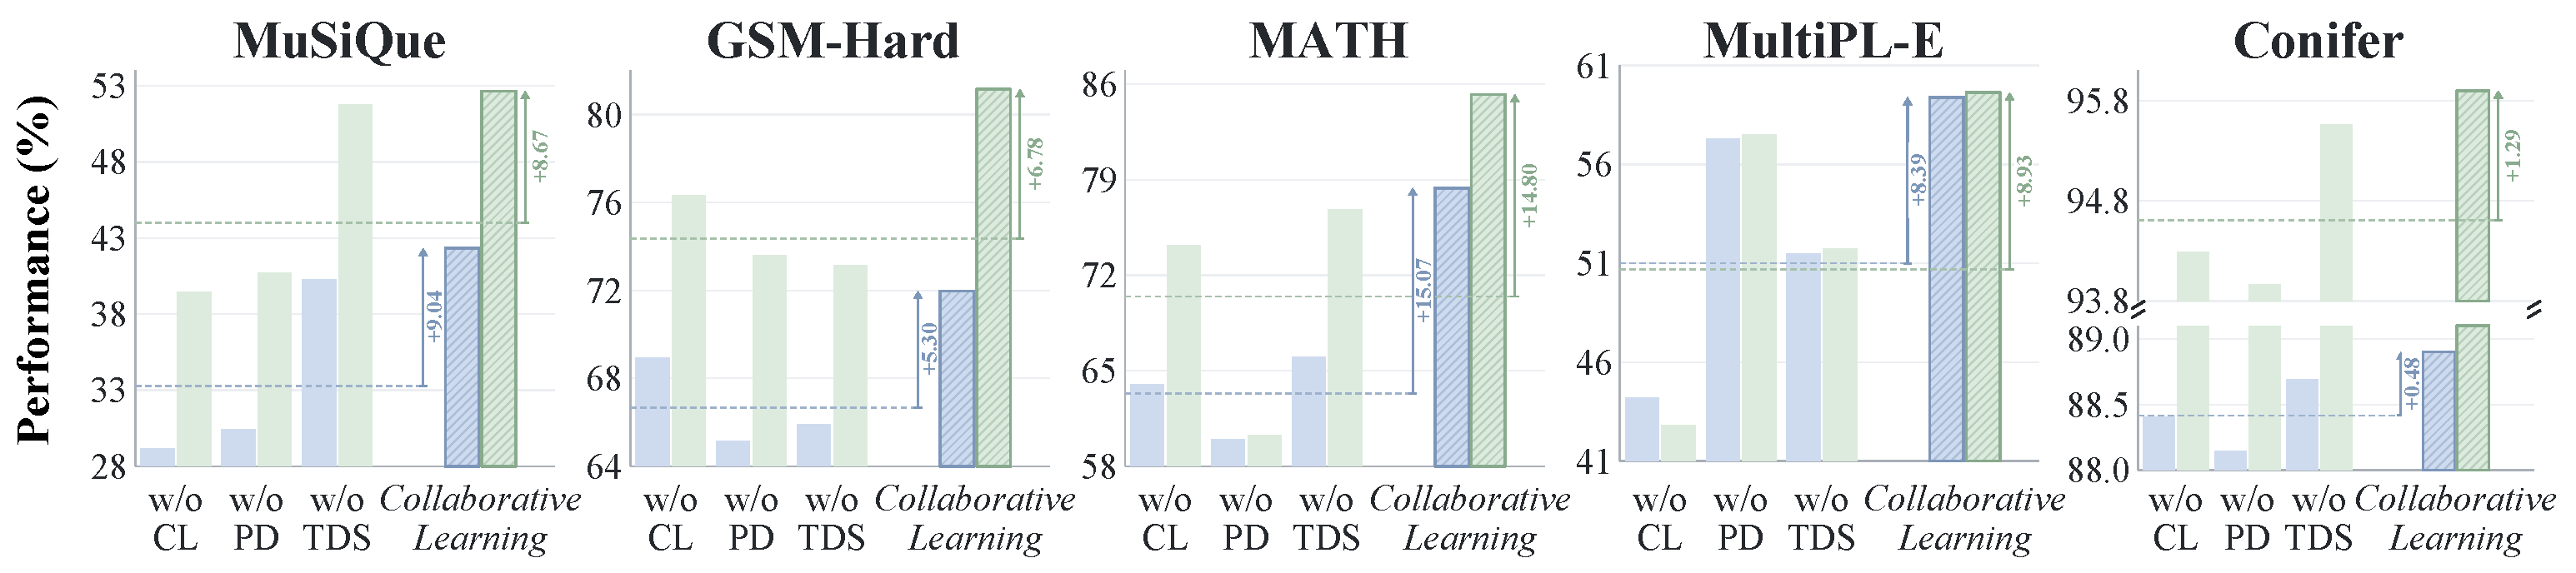
\includegraphics[width=\linewidth]{figures/Figure3.pdf}
\vspace{-1.5em}
\caption{\textbf{Ablation study of the mechanism across five benchmarks.} We compare variants without Protocol Distillation (PD) or the step-level deliberative score (TDS), together with a zero-shot variant that receives no training (w/o CL). Arrows indicate the gain of \textit{collaborative learning} over the arithmetic mean of the available variants. For each benchmark, \raisebox{0.15ex}{\textcolor[RGB]{206,219,239}{\rule{1.3em}{0.8em}}} denotes Acc., Wtd., and Cov., while \raisebox{0.15ex}{\textcolor[RGB]{220,235,221}{\rule{1.3em}{0.8em}}} denotes the corresponding second metric (F1, Mac., or Expl.).}
\label{fig:ablation_results}
\end{figure}
\FloatBarrier

Without protocol distillation, MuSiQue first-answer EM improves from 21.02\% to 25.24\%, yet initially incorrect answers corrected by the final response fall from 594 to 171. Conifer trajectories that pass initially but fail at termination increase from 0.78\% to 2.92\%, while MATH protocol-following failures rise from 16.6\% to 35.0\%. Thus, protocol distillation supports correction and protocol-following rather than merely first-answer accuracy. Removing step-level deliberative scores lengthens MuSiQue trajectories from 3.4 to 3.8 steps while reducing corrections by 18.5\%; GSM-Hard trajectories average 1.4 steps, with no handoff on 66.67\% of questions and seven protocol-following failures. These patterns show that outcome rewards inadequately guide intermediate decisions; process supervision instead separates productive collaboration from redundant or unsafe interactions.


\subsection{How Efficient and Effective Is Collaborative Reasoning?}
\label{sec:efficiency}

Alongside the task-performance gains, our system uses fewer model invocations than MAD, AgentVerse, AFlow, and GPTSwarm~\citep{du2024debate,chen2024agentverse,zhang2025aflow,zhuge2024gptswarm} across all five benchmarks (Figure~\ref{fig:efficiency}). It requires an average of 4.0, 4.1, 1.8, 3.0 and 3.3 invocations per question on MuSiQue, GSM-Hard, MultiPL-E, MATH and Conifer, respectively, corresponding to relative reductions of 39.1\%--84.8\% over these frameworks. Among the compared methods, our system achieves the lowest parameter-weighted output token counts on GSM-Hard, MultiPL-E, MATH, and Conifer, and the third-lowest on MuSiQue. On the four benchmarks where our system achieves the lowest count, its counts are 96.2\%, 58.3\%, 73.1\% and 36.2\% lower, respectively, than those of the lowest-cost baseline under this metric on the corresponding benchmark.

We compare pre- and post-training reasoning-overlap rates. On MuSiQue, the rates for A1, A2, and A3 decrease from 48.3\%, 24.1\%, and 55.2\% to 0.2\%, 0.3\%, and 0.5\%, respectively. On MultiPL-E, they decrease from 34.8\%, 2.3\%, and 17.6\% to 7.4\%, 1.8\%, and 10.7\%. These results suggest that collaborative training reduces repetition in both interaction decisions and reasoning content.

To assess collaborative effectiveness, we further measure correct-answer retention, defined as the proportion of trajectories with a correct final answer among those containing a correct intermediate candidate. Our method achieves retention rates of 80.42\%, 97.94\%, 98.26\%, and 98.00\% on MuSiQue, GSM-Hard, MultiPL-E, and MATH, respectively\footnote{Conifer is excluded because open-ended outputs lack a binary criterion for correct intermediate candidates.}, outperforming all four comparison frameworks. AgentVerse is the strongest baseline on the first three benchmarks, with retention rates of 76.32\%, 95.96\%, and 85.98\%, respectively, while GPTSwarm leads the baselines on MATH at 92.76\%. Our method therefore achieves absolute retention gains of 4.11\%, 1.98\%, 12.28\%, and 5.24\% over the strongest baseline on each benchmark, respectively. These results show that, within each method's own generated trajectories, our system preserves correct candidates through to the final response at a higher rate, with fewer correct answers lost during subsequent interactions.

\begin{figure}[!htbp]
\centering
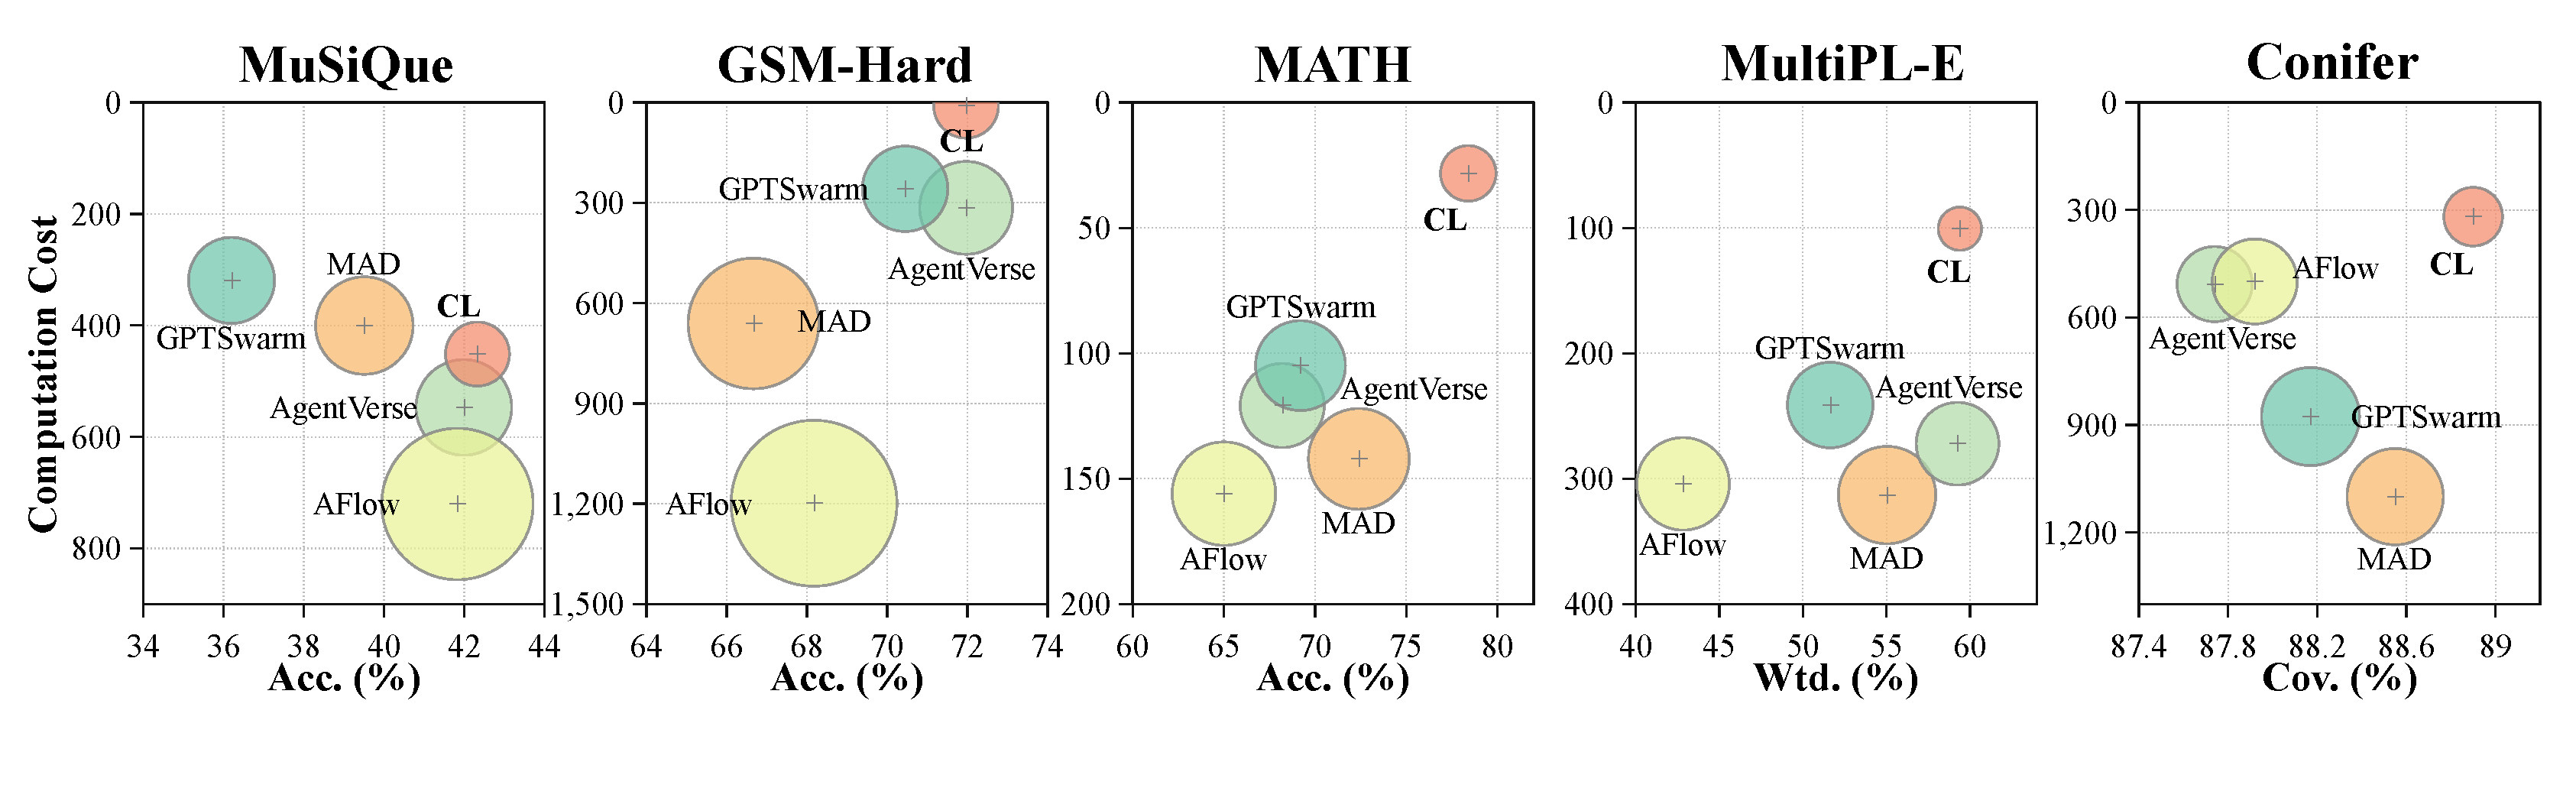
\includegraphics[width=\linewidth]{figures/Figure4.pdf}
\vspace{-1.25em}
\caption[Computation cost versus task performance.]{\textbf{Computation cost versus task performance.} The center of each circle indicates task performance and parameter-weighted output tokens\protect\footnotemark{} for our method and four multi-agent baselines across five benchmarks; its area is proportional to the average number of model invocations.}
\label{fig:efficiency}
\end{figure}
\footnotetext{The parameter-weighted output-token metric is detailed in Appendix~\ref{app:efficiency_metrics}.}
\FloatBarrier

\subsection{What Collaboration Patterns Emerge from Collaborative Learning?}
\label{sec:collaborative_pattern}

\begin{figure}[!htbp]
\centering
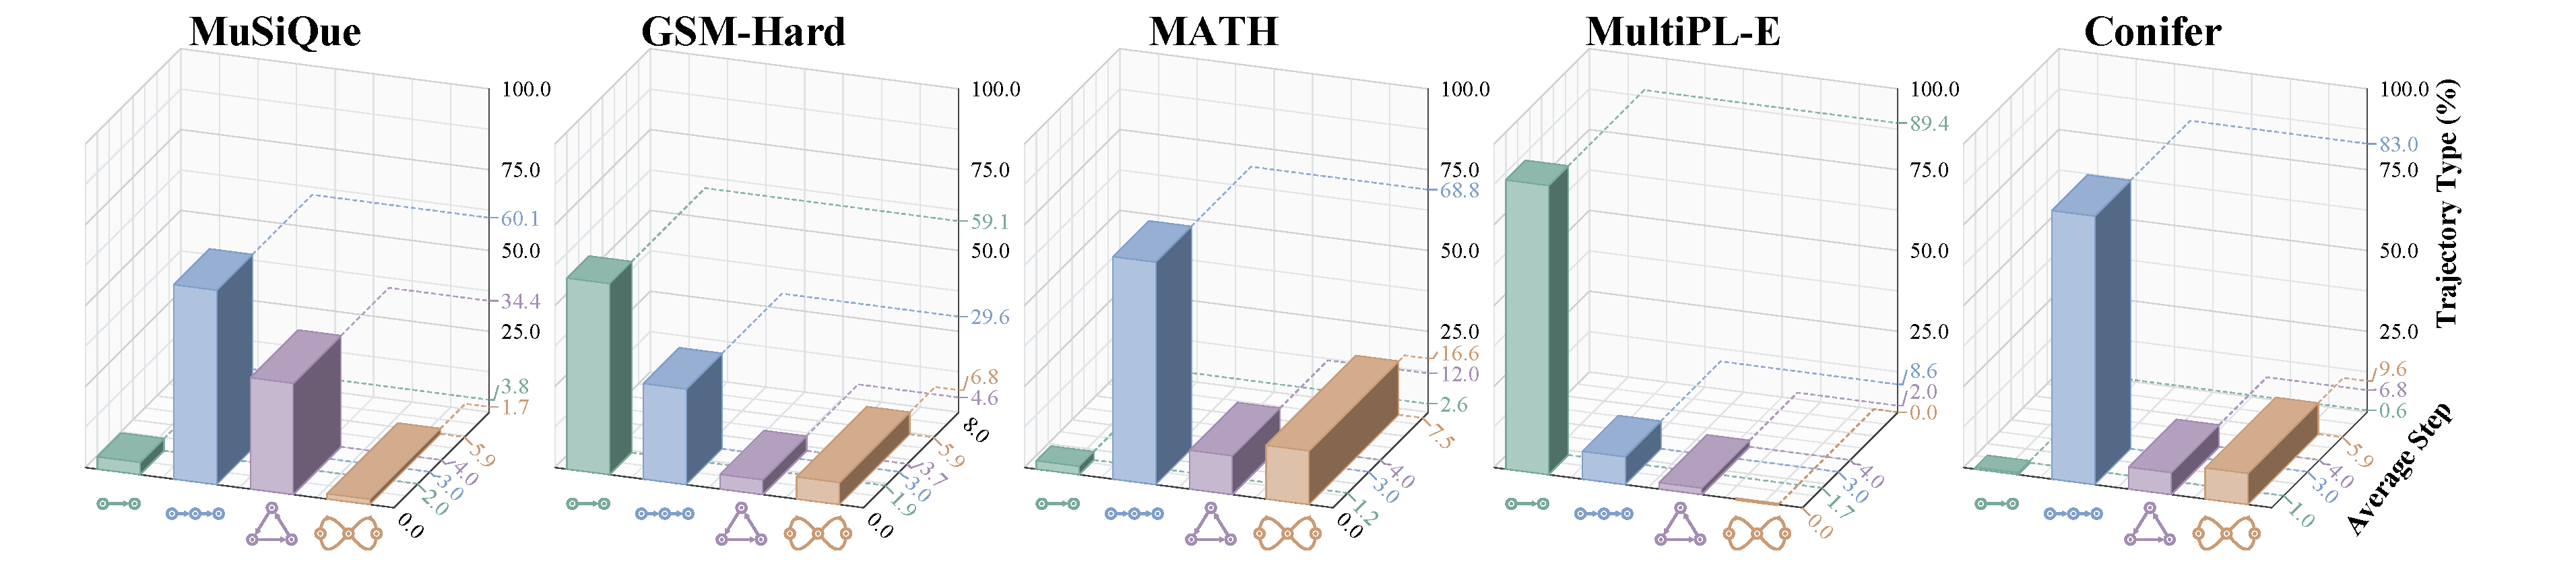
\includegraphics[width=\linewidth]{figures/Figure5.pdf}
\vspace{-1.5em}
\caption{\textbf{Post training interaction topology across tasks.}
\protect\raisebox{-0.15em}{\protect\includesvg[height=1.15em]{figures/logo_short}},
\protect\raisebox{-0.15em}{\protect\includesvg[height=1.15em]{figures/logo_linear}},
\protect\raisebox{-0.15em}{\protect\includesvg[height=1.15em]{figures/logo_cyclic_short}},
and
\protect\raisebox{-0.15em}{\protect\includesvg[height=1.15em]{figures/logo_cyclic_long}}
denote short linear, long linear, short cyclic, and long cyclic trajectories, respectively. Bar height shows the proportion of each trajectory type, while depth shows the average number of interaction steps.}
\label{fig:interaction_topology}
\end{figure}
\FloatBarrier

To examine how training changes the organization of collaboration, we compare interaction topologies and the number of model interaction steps before and after training. We categorize interaction trajectories into four types: short linear, long linear, short cyclic, and long cyclic. In linear trajectories, each model participates at most once; short trajectories have at most two interaction steps, whereas long trajectories have more than two. Cyclic trajectories return to a previously participating model at least once, forming a cycle. For cyclic trajectories, short trajectories have at most four interaction steps, whereas long trajectories have more than four. The proportion of long linear trajectories on MuSiQue increases from 9.18\% to 60.12\%, indicating that training favors linear trajectories with more interaction steps on this task. In contrast, the proportion of long linear trajectories on MultiPL-E decreases from 10.95\% to 8.58\%. On GSM-Hard, the average number of interaction steps in short cyclic trajectories decreases from 4.00 to 3.67, while that on MATH increases from 3.33 to 4.00. Figure~\ref{fig:interaction_topology} visualizes the resulting post-training interaction structures across tasks. These results suggest that training does not uniformly lead to more complex interaction structures or more interaction steps, but instead produces task-dependent patterns of collaboration.


An emerging division of labor is also visible on MuSiQue: Qwen3-4B's answer revision rate increases from 13\% to 69\%, its handoff rate rises from 48\% to 96\%, and its termination rate decreases from 50\% to 4\%, indicating a shift toward intermediate revision and handoff. Qwen3-8B, meanwhile, more frequently provides the final answer, with its share of final answers increasing from 13.0\% to 58.4\%. This division of labor does not constitute a fixed role assignment: on GSM-Hard, Qwen3-4B more frequently provides the final answer, with its share increasing from 34.09\% to 64.39\%. Thus, models develop task-dependent divisions of labor without predefined roles\footnote{Cases in Appendix~\ref{app:case_studies} show how models collaborate through different interaction patterns across tasks.}.



\section{Related Work}
\label{sec:related_work}

\vspace{-1em}

\noindent\textbf{Reasoning in LLMs.}\quad Existing work improves LLM reasoning by eliciting existing capabilities or strengthening them through training~\citep{zhao2026selfdistilled,li2026rise,liu2026spade}. Inference-time methods use chain-of-thought prompting~\citep{wei2022chain}, systematic exploration~\citep{hariri2026regimes,li2026tailsearch}, evaluation~\citep{wu2026stv}, and revision~\citep{yang2026retree}; training-based methods learn from bootstrapped demonstrations~\citep{zelikman2022star,dong2026bird}, distill teacher reasoning~\citep{yang2025supercorrect,liu2026sparse,fu2026onetraining}, or use outcome- and process-level supervision. Yet these methods remain bounded by a single model's knowledge and reasoning biases, leaving blind spots unaddressed and allowing intermediate errors to persist through subsequent reasoning~\citep{xie2026breadth}.


\noindent\textbf{From Single-Model Reasoning to Multi-Model Composition.}\quad These limitations motivate moving beyond single-model reasoning toward multi-model composition, which exploits complementary knowledge and task-specific strengths across models~\citep{yang2026corl,zhang2026hacrl,huot2026meaningful}. Existing approaches select models suited to an input~\citep{ong2025routellm,cao2026scope,feng2026llmrouter,fisch2026pandora}, distribute tasks or subtasks~\citep{agashe2025agents2,chen2026mhgpo}, organize sequential model invocations~\citep{dekoninck2025routing,li2026progrouter}, determine when additional models are needed~\citep{rajib2026gatedmemory,qin2026atlas}, and aggregate candidate outputs~\citep{zhang2026agentrouter}. However, system-level composition does not necessarily constitute collaborative reasoning in which models jointly develop, evaluate, and revise a shared solution.

\noindent\textbf{Multi-Model Collaborative Reasoning.}\quad Collaborative reasoning directly addresses how models jointly develop solutions through interaction. Existing approaches range from hand-designed roles and protocols to optimized workflows~\citep{hu2025adas,zhou2026mass,lee2026mega,koh2026graft} and learned collaborative policies~\citep{xue2026comas,zhang2026metaagentx}. Representative systems, however, often retain an explicitly prescribed division of labor~\citep{zhao2026strongermas,feng2026drmas,ding2026apex}. In contrast, we train heterogeneous small models to collaborate without predefined roles under a total parameter budget comparable to that of a single large model.

\vspace{-0.5em}

\section{Conclusion}

\looseness=-1
We introduced a three-stage collaborative learning method: model slicing, protocol distillation, and pyramid supervision. Model slicing replaces a large model with smaller heterogeneous models, while protocol distillation and pyramid supervision train them to collaborate without predefined roles. Across four task categories, our method matches or outperforms the original model and multi-agent baselines under a comparable total parameter budget. Training reduces redundant interactions, improves correct-answer retention, and induces task-dependent collaboration patterns. These results show that heterogeneous models can learn to collaborate without predefined roles or workflows, while step-level feedback helps them develop differentiated functions aligned with their capabilities.

\section{Discussion}

\noindent\textbf{Limitations.}\quad Our study is currently limited to three model sizes and five benchmarks, so whether the observed gains extend to larger model pools, longer interaction horizons, or unseen task distributions remains to be established. Pyramid supervision also depends on the quality of the inspector and task-specific evaluators, whose biases may affect step-level feedback. Finally, comparable total parameter counts do not imply equivalent computational cost, as collaborative inference may introduce additional latency and memory overhead not fully captured by our parameter-weighted output-token metric.


\noindent\textbf{Future Work.}\quad Future work will further examine how collaborative learning generalizes to unseen tasks, larger model pools, and longer interaction horizons. Incorporating multiple independent inspectors or uncertainty-aware aggregation may further improve the robustness of supervision.

\section*{AI use statement}

We used AI tools to assist with drafting and polishing the manuscript, writing portions of the experimental code, preparing figures, and searching for literature. The authors reviewed and revised the AI-assisted text and figures, and modified, verified, and tested the AI-assisted code. For the literature, AI tools served only as an aid to searching; the authors independently selected, reviewed, organized, and synthesized the relevant publications. We take full responsibility for the content of this work, including all text, claims, and artifacts produced with the assistance of generative AI.

\bibliography{iclr2027_conference}
\bibliographystyle{iclr2027_conference}

\clearpage
\appendix
\section*{Appendix}
\colorlet{appendixHeader}{CadetBlue!20}
\colorlet{appendixStripe}{gray!10}
\colorlet{appendixInk}{black}
\colorlet{appendixRule}{black}
\newcommand{\appendixHeading}[1]{\textcolor{appendixInk}{\textbf{#1}}}

\section{Overview of the Training Algorithm}
\label{app:algorithm}

Algorithm~\ref{alg:collaboration} summarizes the two training stages: protocol distillation and pyramid supervision. Let $\mathcal{M}=\{M_1,\ldots,M_N\}$ denote the heterogeneous agent pool. The teacher model $M^\star$, selected as the largest model in this pool by parameter count, generates trajectories for protocol distillation; we use Qwen3-8B in our experiments. The original large model $M_L$ (Qwen3-14B) serves as the inspector $\mathcal{J}$ during training on all five datasets but is not deployed during collaborative inference.

Let $\mathcal{Q}_{\mathrm{distill}}$ and $\mathcal{Q}_{\mathrm{pyramid}}$ denote the task inputs used for protocol distillation and pyramid supervision, respectively. For each task $q$, we use the trajectory notation $\tau=(z_1,\ldots,z_T)$ with $z_t=(i_t,x_t,y_t,a_t)$ defined in Section~\ref{sec:collaborative_reasoning}, where $x_t$ contains $q$ and the preceding interaction history. The training target $o_t$ is the full serialized response at step $t$, including its reasoning, answer, and interaction fields. The distribution $P_{\mathcal{M}}(\tau\mid q)$ is induced by the agent pool and its interaction protocol. During protocol distillation, a permutation $\pi$ is sampled uniformly from $S_N$, the set of permutations of the $N$ agent identities, and used to remap identities consistently throughout each teacher trajectory. The retained, remapped steps form the supervised dataset $\mathcal{D}_{\mathrm{distill}}$. During pyramid supervision, the inspector assigns a score $s_t^{\mathrm{ins}}$ to each step. Task feedback and inspection scores determine the training weight $r_t$ according to Appendix~\ref{app:training}. For each agent $M_i$, the dataset $\mathcal{D}_i$ contains $(x_t,o_t,r_t)$ from steps with $i_t=i$, so each model is optimized using only its own actions.

\begingroup
\makeatletter
\let\appendixOriginalRuled\fs@ruled
\renewcommand{\fs@ruled}{%
  \appendixOriginalRuled
  \def\@fs@capt##1##2{%
    \begingroup
    \setlength{\fboxsep}{2pt}%
    \noindent\colorbox{appendixHeader}{%
      \parbox{\dimexpr\linewidth-2\fboxsep\relax}{%
        \color{appendixInk}\floatc@ruled{##1}{##2}}}\par
    \endgroup
  }%
  \def\@fs@pre{{\color{appendixRule}\hrule height.8pt depth0pt}\kern2pt}%
  \def\@fs@mid{\kern2pt{\color{appendixRule}\hrule}\kern2pt}%
  \def\@fs@post{\kern2pt{\color{appendixRule}\hrule}}%
}
\makeatother
\begin{algorithm}[H]
\caption{Protocol Distillation and Pyramid Supervision for Heterogeneous Collaboration}
\label{alg:collaboration}
\small
\begin{algorithmic}[1]
\Require Agent pool $\mathcal{M}$; largest model in the pool $M^\star$; task collections $\mathcal{Q}_{\mathrm{distill}},\mathcal{Q}_{\mathrm{pyramid}}$; inspector $\mathcal{J}$; task-specific reward configuration
\State Construct homogeneous teacher MAS $\mathcal{M}_{\mathrm{teacher}}=\{M_1^\star,\ldots,M_N^\star\}$
\State \appendixHeading{Stage I: Protocol Distillation}
\State $\mathcal{D}_{\mathrm{distill}}\gets\emptyset$
\For{$q\in\mathcal{Q}_{\mathrm{distill}}$}
  \State Roll out teacher trajectory $\tau\sim P_{\mathcal{M}_{\mathrm{teacher}}}(\tau\mid q)$
  \State Retain examples satisfying the task-specific data filters
  \State Sample identity permutation $\pi\sim\mathrm{Uniform}(S_N)$
  \State Apply $\pi$ consistently to all agent identities in $\tau$
  \State Add remapped steps to $\mathcal{D}_{\mathrm{distill}}$
\EndFor
\For{$i=1,\ldots,N$}
  \State Distill protocol behavior into $M_i$ using its corresponding steps in $\mathcal{D}_{\mathrm{distill}}$
\EndFor
\State \appendixHeading{Stage II: Pyramid Supervision}
\For{each training iteration}
  \State $\mathcal{D}_1,\ldots,\mathcal{D}_N\gets\emptyset$
  \For{$q\in\mathcal{Q}_{\mathrm{pyramid}}$}
    \State Collect or retrieve a heterogeneous trajectory $\tau$ for $q$
    \State Compute task reward $r_{\mathrm{task}}$
    \State Obtain inspection scores $\{s_t^{\mathrm{ins}}\}_{t=1}^T$ from $\mathcal{J}(q,\tau)$
    \For{$t=1,\ldots,T$}
      \State Compute $r_t$ using task feedback and inspection scores (Appendix~\ref{app:training})
      \State Add $(x_t,o_t,r_t)$ to $\mathcal{D}_{i_t}$
    \EndFor
  \EndFor
  \For{$i=1,\ldots,N$}
    \State Update $M_i$ with $\mathcal{D}_i$ using reward-weighted optimization
  \EndFor
\EndFor
\State \Return Trained heterogeneous agents $\mathcal{M}=\{M_1,\ldots,M_N\}$
\end{algorithmic}
\end{algorithm}
\endgroup

\section{Interaction and Inspection Protocol}
\label{app:protocol}

This section details response requirements, inspector inputs, and task-specific scoring criteria.

\FloatBarrier
\subsection{Response Schema and Field Requirements}
\label{app:output_schema}
Following the interaction protocol defined in Section~\ref{sec:collaborative_reasoning}, each agent produces a serialized response with the following fields and action-specific requirements at every collaboration step.

\noindent\textbf{Field requirements.}
\begin{itemize}
    \item \texttt{reasoning}: the current step's explanation or verification.
    \item \texttt{tentative\_answer}: the current candidate---a MuSiQue answer, a GSM-Hard number, a MATH expression, a Conifer response, or code in its designated field.
    \item \texttt{action}: the serialized control decision corresponding to $a_t$.
    \item \texttt{handoff\_target}: a permitted recipient ID within the model pool for the next handoff.
    \item \texttt{handoff\_note}: the specific issue the recipient should check.
    \item \texttt{confirmed\_answer}: the final answer for \texttt{terminate}, and null otherwise. For termination, the handoff fields remain null because no recipient is selected.
\end{itemize}
\FloatBarrier
\subsection{Inspector Inputs}

\paragraph{Inspector model.}
Qwen3-14B serves as the shared inspector for all five datasets.

\paragraph{Input visibility.}
Table~\ref{tab:app-inspector-inputs} summarizes inspector inputs across tasks.

\begin{table}[!htbp]
\centering
\caption{Information Available to the Inspector.}
\label{tab:app-inspector-inputs}
\small
\setlength{\tabcolsep}{3pt}
\renewcommand{\arraystretch}{1.15}
\begin{tabular}{@{\hspace{\tabcolsep}}p{0.14\linewidth}p{0.15\linewidth}p{0.15\linewidth}p{0.15\linewidth}p{0.16\linewidth}p{0.15\linewidth}@{\hspace{\tabcolsep}}}
\toprule
\rowcolor{appendixHeader}
\appendixHeading{Information} & \appendixHeading{MuSiQue} & \appendixHeading{GSM-Hard} & \appendixHeading{MATH} & \appendixHeading{MultiPL-E} & \appendixHeading{Conifer} \\
\midrule
Task context & Question and reference paragraphs & Problem statement & Problem statement & Source prefix and language & Instruction and parsed constraints \\
\midrule
\rowcolor{appendixStripe}
Reference information & Gold answer & Gold numeric answer & Gold mathematical answer & No reference code supplied & Reference response for audit \\
\midrule
Candidate and final outputs & Tentative and final answers & Tentative and confirmed answers & Tentative and confirmed answers & Tentative and confirmed code completions & Response drafts and final response \\
\midrule
\rowcolor{appendixStripe}
Agent identity & Agent ID per step & Agent ID per step & Agent ID per step & Agent ID per step & Agent ID per step \\
\midrule
Step sequence & All recorded steps and actions & All recorded steps and actions & All recorded steps and actions & All recorded steps and actions & All recorded steps and actions \\
\midrule
\rowcolor{appendixStripe}
Reasoning text & Up to 400 characters per step & Untruncated reasoning & Untruncated reasoning & Up to 1,200 characters per step & Up to 1,200 characters per step \\
\bottomrule
\end{tabular}
\end{table}

\FloatBarrier
\subsection{Task-Specific Inspection}

The inspector evaluates reasoning quality and the usefulness of each step's interaction decision. Table~\ref{tab:app-rubric} summarizes the scoring criteria for all five datasets used in our experiments.

\begin{table}[!htbp]
\centering
\caption{Scoring Dimensions and Criteria by Dataset.}
\label{tab:app-rubric}
\small
\setlength{\tabcolsep}{3pt}
\renewcommand{\arraystretch}{1.15}
\begin{tabular}{@{\hspace{\tabcolsep}}p{0.14\linewidth}p{0.20\linewidth}p{0.16\linewidth}p{0.42\linewidth}@{\hspace{\tabcolsep}}}
\toprule
\rowcolor{appendixHeader}
\appendixHeading{Dataset} & \appendixHeading{Dimensions} & \appendixHeading{Score range} & \appendixHeading{Criteria} \\
\midrule
MuSiQue & Reasoning; action & $[-1,1]$, continuous & Evidence citations and multi-hop reasoning; supported correction and verification; penalties for regression and redundant interaction. \\
\midrule
\rowcolor{appendixStripe}
GSM-Hard & Process & $[-1,1]$, step size $0.5$ & Correct, independently checkable arithmetic and appropriate actions; penalties for weak verification, misleading computation, and unsafe stopping. Incorrect candidates cannot receive positive scores. \\
\midrule
MATH & Process & $[-1,1]$, step size $0.5$ & Correct mathematical reasoning and useful verification or correction; penalties for misleading work, regression, and unsafe stopping. Incorrect candidates cannot receive positive scores. \\
\midrule
\rowcolor{appendixStripe}
MultiPL-E & Reasoning; action & $[-1,1]$, continuous & Implementation logic, edge cases, syntax, and completion boundaries; useful bug fixes and code audits; penalties for invalid completions and unsupported confirmation. \\
\midrule
Conifer & Reasoning; action; content; final quality & Step: $[-1,1]$; final: $[0,1]$ & Constraint analysis, draft quality, and useful handoff or stopping decisions; penalties for repetition, premature stopping, and regression. Final quality evaluates the submitted response. \\
\bottomrule
\end{tabular}
\end{table}

\FloatBarrier
\section{Training and Inference Details}
\label{app:training}

\subsection{Task Rewards and Training Weights}

Let $S(q,\tau)\in[0,1]$ denote the task score and $s_t^{\mathrm{ins}}\in[-1,1]$ the inspection score. For MuSiQue and Conifer, the training reward is
\begin{equation}
 r_{\mathrm{task}}=2S(q,\tau)-1,
 \qquad
 r_t=\alpha r_{\mathrm{task}}+(1-\alpha)s_t^{\mathrm{ins}}
 \label{eq:app-mixed-reward}
\end{equation}
with $\alpha=0.6$ for MuSiQue and $\alpha=0.5$ for Conifer. The corresponding task-feedback coefficients in the base reward are $\alpha=0.35$ for GSM-Hard, $\alpha=0.35$ for MATH, and $\alpha=0.3$ for MultiPL-E.

\subsection{Agent-Wise Optimization}

For context $x$ and serialized response $o$, let $\ell_{\mathrm{all}}(x,o)$ denote the mean log probability over response tokens. The signed reward-weighted objective follows a score-function policy-gradient form~\citep{williams1992simple}:
\begin{equation}
 \mathcal{L}_i
 =-\mathbb{E}_{(x,o,r)\sim\mathcal{D}_i}\!\left[
 \mathbb{I}[r>0]r\ell_{\mathrm{all}}(x,o)
 +\mathbb{I}[r<0]r\ell_{\mathrm{neg}}(x,o)
 \right]
 +\beta\,\mathbb{E}_{(x,o,r)\sim\mathcal{D}_i}
 \left[\overline{D}_{\mathrm{KL}}(x,o)\right]
 \label{eq:app-rwr}
\end{equation}
where $\overline{D}_{\mathrm{KL}}$ is the mean token-level KL divergence to the frozen SFT reference~\citep{ziegler2019finetuning}.

\subsection{Hardware and LoRA Configuration}

Training uses $8\times$ NVIDIA A800-SXM4-80GB GPUs with a separate LoRA adapter~\citep{hu2022lora} per model and frozen base parameters. The adapters use rank 64, scaling alpha 64, and dropout 0.05. LoRA targets the attention projections \texttt{q\_proj}, \texttt{k\_proj}, \texttt{v\_proj}, and \texttt{o\_proj}, and the MLP projections \texttt{gate\_proj}, \texttt{up\_proj}, and \texttt{down\_proj} in every agent-specific adapter.

\FloatBarrier
\section{Baseline Implementations and Comparison Protocol}
\label{app:baselines}

This section details the implementation and evaluation settings of each baseline. Single-agent controls are Qwen3-14B~\citep{yang2025qwen3} and Qwen3-14B SE-RL. Homogeneous controls are an untrained MAS of three Qwen3-8B agents (Homo. MAS) and a collaboratively trained system of three Qwen3-4B agents (Homo. CL). Established multi-agent comparisons are MAD, AgentVerse, AFlow, and GPTSwarm~\citep{du2024debate,chen2024agentverse,zhang2025aflow,zhuge2024gptswarm}; multi-agent reinforcement-learning comparisons are MAGRPO, MAPoRL, and AT-GRPO~\citep{liu2026collaboration,park2025maporl,zhao2026strongermas}. All use Qwen3 models with the assignments and task-specific configurations detailed below.

\subsection{Single-Agent and Homogeneous Controls}

\paragraph{Qwen3-14B.}
We use the original Qwen3-14B checkpoint as a single-agent baseline for every task.

\paragraph{Qwen3-14B SE-RL.}
We initialize the policy and evaluator from Qwen3-14B, freeze the evaluator during training, and use it to score the policy's generated trajectories.

\paragraph{Homogeneous MAS.}
We use three original Qwen3-8B checkpoints as agents for multi-step collaborative reasoning under the shared interaction protocol used by our system.

\paragraph{Homogeneous collaborative learning (Homo. CL).}
We use the same training and evaluation configuration as CL, replacing its heterogeneous Qwen3-1.7B, Qwen3-4B, and Qwen3-8B model pool with three independently adapted Qwen3-4B agents (12B total).

\subsection{MAD}

MAD organizes reasoning as a multi-round debate in which multiple agents first solve a task independently and then revise their answers after observing the other agents' responses from the preceding round~\citep{du2024debate}. After the final round, the agents' answers are aggregated by majority vote. Our implementation follows MAD's core workflow of independent initial reasoning, iterative peer-conditioned revision, and majority-vote aggregation at test time.

We deploy three debaters using Qwen3-1.7B, Qwen3-4B, and Qwen3-8B, matching the model pool of our heterogeneous MAS. With three total rounds, the nominal cost is nine agent calls per problem, excluding retries. This preserves MAD's three-agent debate and majority-vote structure while making minor adaptations for our Qwen3-based comparison setting.

\subsection{AgentVerse}

AgentVerse recruits three task-specific specialists to generate responses and uses an evaluator to determine whether another iteration is needed~\citep{chen2024agentverse}. The default maximum is three iterations. The evaluator scores the team's responses on a 0--10 scale, with early stopping at a score of at least 8. It receives the task input and agent responses, not a gold answer. The collective answer uses normalized voting with tie handling. This implementation follows AgentVerse's core workflow of expert recruitment, collaborative decision-making, and evaluation-guided iteration.

The three specialist agents use Qwen3-1.7B, Qwen3-4B, and Qwen3-8B, while both the recruiter and evaluator use Qwen3-8B by default. With one recruitment call and four calls per iteration, the nominal range is 5--13 calls, excluding retries. This preserves AgentVerse's separation of specialist, recruitment, and evaluation calls while adapting the backbones and team size to the shared setting.

\subsection{AFlow}

AFlow automates agentic workflow generation by using an optimizer model to propose executable workflows composed of reusable operators, evaluating candidate workflows on task examples, and iteratively refining them through search~\citep{zhang2025aflow}. The selected workflow is then frozen and executed independently at evaluation time. Our implementation follows AFlow's core paradigm of workflow search, execution-based evaluation, and deployment of the selected workflow.

We use Qwen3-14B as the workflow optimizer. During workflow execution, solving calls rotate across Qwen3-1.7B, Qwen3-4B, and Qwen3-8B, while candidate selection and answer extraction use Qwen3-8B by default. Workflow search uses 20 examples and 20 iterations. The optimizer is not invoked during evaluation, preserving AFlow's search-then-execute design.

\subsection{GPTSwarm}

GPTSwarm represents a multi-agent system as an optimizable computational graph, where typed language-model nodes perform specialized operations and directed edges determine how intermediate outputs are exchanged~\citep{zhuge2024gptswarm}. The original method optimizes graph connectivity, while graph execution propagates information toward a designated output node. Our implementation retains GPTSwarm's core graph-structured execution and typed-node composition.

The GPTSwarm-Fixed adaptation executes a fixed seven-node directed acyclic graph: two input/output nodes, three chain-of-thought nodes, one debate node, and one final aggregator. The default routing maps input/output nodes to the 1.7B model, chain-of-thought nodes to the 4B model, and debate/aggregation nodes to the 8B model. Using the original task input, the aggregator synthesizes one answer from its predecessors rather than taking a majority vote.

\subsection{MAGRPO}

We adapt MAGRPO~\citep{liu2026collaboration} to three agents backed by Qwen3-1.7B, Qwen3-4B, and Qwen3-8B, each with an independent LoRA adapter. Training samples groups of eight collaborative episodes and computes episode-relative advantages, with dynamic sampling used to maintain usable groups. The clipped objective uses clip ratio 0.2, advantage clipping at 4, and sequence-mean reduction. The KL coefficient is 0.02 except on MultiPL-E, where it is zero. All three policies use learning rate $5{\times}10^{-6}$. Evaluation runs two synchronous rounds.

\subsection{MAPoRL}

We implement MAPoRL~\citep{park2025maporl} with Qwen3-1.7B, Qwen3-4B, and Qwen3-8B agents and independent LoRA adapters. Each collaborative episode contains three rounds with one proposal from each agent per round. Training uses reward discount 0.3, PPO clip ratio 0.2, KL coefficient 0.002, one PPO epoch, and eight minibatches, with learning rate $10^{-5}$.

\subsection{AT-GRPO}

We use the agent-and-turn grouped optimization procedure of AT-GRPO~\citep{zhao2026strongermas}. The three Qwen3-1.7B, Qwen3-4B, and Qwen3-8B policies have independent LoRA adapters and use spine-tree sampling with three training rounds and group size eight. The clipped objective uses ratio 0.2, KL coefficient 0.02, advantage clipping at 4, and sequence-mean reduction. The A1/A2/A3 learning rates are $2{\times}10^{-5}$, $1.5{\times}10^{-5}$, and $10^{-5}$, respectively. Evaluation uses four synchronous rounds on MuSiQue, GSM-Hard, MATH, and Conifer, and three rounds on MultiPL-E.

\FloatBarrier
\s.}
For each dataset, our method and all baselines are evaluated using the same task-specific evaluatoretcounter{subsection}{9}
\subsection{Conifer Evaluation Metrics}
\label{app:conifer_metrics}

For Conifer, we report two deterministic constraint-compliance metrics computed from each final response. The evaluator first applies a conservative parser to the instruction. For Coverage, it retains numbered requirements containing 2--12 words and at most 120 characters. For Explicit, it extracts mechanically verifiable constraints comprising response presence; requested output formats (bulleted, ordered, or general lists, tables, code, and paragraphs); word, sentence, and list-item limits; and quoted terms that must appear in the response. Neither uses inspectors or references.

Let $a_q$ be the final response for example $q$, $\mathcal{R}_q$ the set of parsed numbered requirements, and $\mathcal{T}(s)$ the set of unique lower-cased, non-stopword alphanumeric tokens in text $s$, allowing apostrophes, underscores, and hyphens within tokens. For an individual requirement $r$, its lexical coverage is
\begin{equation}
 c(a_q,r)=
 \begin{cases}
 1, & |\mathcal{T}(r)|=0,\\
 \dfrac{|\mathcal{T}(r)\cap\mathcal{T}(a_q)|}{|\mathcal{T}(r)|}, & \text{otherwise}.
 \end{cases}
\end{equation}
The per-example Coverage score is
\begin{equation}
 \operatorname{Cov}_q=
 \begin{cases}
 1, & |\mathcal{R}_q|=0,\\
 \dfrac{1}{|\mathcal{R}_q|}\displaystyle\sum_{r\in\mathcal{R}_q}c(a_q,r), & \text{otherwise}.
 \end{cases}
\end{equation}
Thus, Coverage measures the average fraction of each parsed requirement's content tokens that appears in the final response; it is a lexical recall measure rather than a semantic correctness judgment.

For Explicit, let $\mathcal{B}_q$ be the set containing the response-presence check and every mechanically testable constraint extracted for example $q$, and let $b(a_q)\in\{0,1\}$ indicate whether check $b$ passes. The per-example score is
\begin{equation}
 \operatorname{Expl}_q=
 \frac{1}{|\mathcal{B}_q|}\sum_{b\in\mathcal{B}_q} b(a_q).
\end{equation}
All checks receive equal weight. Format and required-term checks use pattern or case-insensitive substring matching, while count constraints compare the measured numbers of words, sentences, or list items with the requested limits. Finally, for $N$ evaluated responses, the reported table entries are $100N^{-1}\sum_q\operatorname{Cov}_q$ and $100N^{-1}\sum_q\operatorname{Expl}_q$. All evaluation items, including unsuccessful predictions, remain in the denominator for every reported aggregate.

\FloatBarrier
\section{Additional Analyses}
\label{app:analysis}

\subsection{Efficiency and Behavioral Metrics}
\label{app:efficiency_metrics}

\paragraph{Amortized parameter-weighted output-token cost.}
We quantify computation cost using amortized parameter-weighted output tokens. This measure combines output tokens generated while solving evaluation problems with an amortized share of the output tokens generated during workflow search. The shared normalization constant is $1.7+4+8+14=27.7$ (in billions), corresponding to the four nominal model sizes used across methods. For a given method and benchmark, the per-problem cost is
\begin{equation}
 C_{\mathrm{out}}(q)
 =\sum_{c\in\mathcal{C}_{\mathrm{eval}}(q)}
   \frac{B_{m(c)}}{27.7}\,L_c^{\mathrm{out}}
 +\frac{1}{N_{\mathrm{eval}}}
  \sum_{c\in\mathcal{C}_{\mathrm{search}}}
   \frac{B_{m(c)}}{27.7}\,L_c^{\mathrm{out}}
 \label{eq:app-weighted-tokens}
\end{equation}
where $B_{m(c)}$ is the nominal parameter count, in billions, of the model producing generation $c$, and $L_c^{\mathrm{out}}$ is the corresponding recorded output-token count. The set $\mathcal{C}_{\mathrm{eval}}(q)$ contains all model generations included during evaluation for problem $q$, including those arising from retries, meta-model evaluations, aggregation, and separate bootstrap solvers. For AFlow, $\mathcal{C}_{\mathrm{search}}$ contains the generations from one recorded workflow search, including those produced by the 14B optimizer and the 1.7B/4B/8B executors used to evaluate candidate workflows. This search cost is divided across the $N_{\mathrm{eval}}$ problems in the evaluation run, not the search examples. Methods without workflow search have $\mathcal{C}_{\mathrm{search}}=\emptyset$. Reported means combine evaluation and search token totals, apply the model weights, and divide by $N_{\mathrm{eval}}$ within each benchmark.

AFlow's 14B optimizer contributes only through the search term, not evaluation-time workflow execution. The metric includes amortized search but excludes training rollouts, teacher generation, training-time inspection, parameter optimization, and offline evaluator replay. It jointly accounts for model size and generated output length. The common normalization does not affect cost ratios, and the amortized search cost per problem decreases as the evaluation set grows.

\paragraph{Reasoning overlap.}
The coordination analysis measures lexical overlap on adjacent steps in which the source agent hands off to the agent that acts next. For receiving agent $i$, the overlap rate is
\begin{equation}
 O_i(\delta)=
 \frac{\sum_{(u,v)\in\mathcal{H}_i}
  \mathbb{I}[\operatorname{ROUGE\!\text{-}\!L}_{F_1}(y_u,y_v)\geq\delta]}
 {|\mathcal{H}_i|}
 \label{eq:app-overlap}
\end{equation}
where $\mathcal{H}_i$ is the set of eligible handoffs received by $i$. This is a threshold-exceedance rate, not a mean similarity score or an embedding-based redundancy metric. Its value depends on the threshold $\delta$, text preprocessing, and the set of valid handoff pairs. Low lexical overlap alone does not prove useful complementary reasoning: an unrelated response can also have low overlap.

\paragraph{Correct-answer discovery and retention.}
Let $\mathcal{V}_q$ be the method-specific set of extracted intermediate candidate answers, and let $g_q(v)$ indicate correctness under the benchmark's grader. Define
\begin{equation}
 D_q=\mathbb{I}[\exists v\in\mathcal{V}_q:g_q(v)=1],
 \qquad
 \mathrm{Discovery}=\frac{\sum_q D_q}{|\mathcal{Q}_{\mathrm{eval}}|},
 \qquad
 \mathrm{Retention}=\frac{\sum_q D_q g_q(\widehat{a}_q)}{\sum_q D_q}
 \label{eq:app-retention}
\end{equation}
Retention is undefined if no correct candidate is discovered. The candidate set $\mathcal{V}_q$ contains intermediate proposals, which are distinct from final aggregation outputs. Differences in extraction coverage can affect cross-method comparisons. A final answer can sometimes be correct even when the extractor finds no correct intermediate candidate, so discovery multiplied by retention need not equal final accuracy. Retention measures preservation of available correct answers; it does not by itself establish the causal mechanism responsible for a performance gain.

\subsection{Self-Evaluation Bias of the 14B Inspector}
\label{app:inspector_bias}

We compare Qwen3-14B inspection scores for heterogeneous-MAS and SE-RL trajectories. Table~\ref{tab:app-inspector-bias} reports mean scores and the share of paired questions favoring the self-generated trajectory.

\begin{table}[!htbp]
\centering
\caption{Qwen3-14B inspection scores for heterogeneous MAS and self-generated SE-RL trajectories. The final column reports the proportion of paired questions on which the self-generated trajectory scores higher than its paired heterogeneous-MAS trajectory.}
\label{tab:app-inspector-bias}
\small
\setlength{\tabcolsep}{4pt}
\renewcommand{\arraystretch}{1.15}
\begin{tabular}{@{\hspace{\tabcolsep}}p{0.20\linewidth}p{0.22\linewidth}p{0.24\linewidth}p{0.24\linewidth}@{\hspace{\tabcolsep}}}
\toprule
\rowcolor{appendixHeader}
\appendixHeading{Dataset} & \appendixHeading{MAS score} & \appendixHeading{Self-generated score} & \appendixHeading{Questions with higher self score} \\
\midrule
MuSiQue & 0.0194 & 0.8692 & 97.25\% \\
\midrule
\rowcolor{appendixStripe}
GSM-Hard & 0.0921 & 0.7991 & 93.26\% \\
\midrule
MultiPL-E-8Lang & 0.6381 & 0.8283 & 90.05\% \\
\midrule
\rowcolor{appendixStripe}
MATH & 0.1054 & 0.4911 & 80.37\% \\
\midrule
Conifer & 0.7643 & 0.8715 & 77.27\% \\
\bottomrule
\end{tabular}
\end{table}

Across all five datasets, the inspector assigns higher mean scores to self-generated trajectories. The paired comparison shows the same asymmetry: self-generated trajectories score higher on 77.27\% to 97.25\% of questions, depending on the dataset in the paired evaluation.

\subsection{Qualitative Analysis of Collaboration Patterns}
\suppressfloats[t]

The two most frequent interaction paths after training are the following:
\begin{equation}
 A_1\rightarrow A_2\rightarrow A_3,
 \qquad
 A_1\rightarrow A_2\rightarrow A_3\rightarrow A_1
\end{equation}
with frequencies of 60.12\% and 34.22\%, respectively. Together they account for 94.34\% of the analyzed trajectories. Both paths involve all three models, while the second returns control to the initial agent after the other two have contributed. This concentration indicates a small set of recurrent interaction patterns. Routing alone does not establish functional specialization, which depends on step content and answer transitions rather than agent order in isolation.

Answer transitions provide a complementary view of these patterns. A wrong-to-correct transition indicates correction, while preserving a correct candidate through later steps indicates retention. A correct-to-wrong transition indicates regression. These transitions do not alone establish independent verification, which also depends on the reasoning content. Scheduler-forced handoffs and minimum-participation rules further constrain the paths independently of model-generated choices.

Section~\ref{app:case_studies} examines these distinctions through matched trajectory comparisons.

\FloatBarrier
\section{Case Studies}
\label{app:case_studies}
\raggedbottom

\colorlet{caseStudyBackground}{appendixHeader!35!white}
\definecolor{caseStudyAccent}{HTML}{887B9C}
\colorlet{caseTranscriptHeader}{appendixHeader}
\colorlet{caseTranscriptMeta}{appendixStripe}
\colorlet{caseTranscriptBody}{white}
\colorlet{caseTranscriptInk}{appendixInk}
\colorlet{caseTranscriptRule}{appendixRule}
\definecolor{caseTranscriptEmphasis}{HTML}{8C5142}
\newcommand{\caseTranscriptHeading}[1]{%
  \rowcolor{caseTranscriptHeader}%
  \textcolor{caseTranscriptInk}{\textbf{Step / action}} &
  \textcolor{caseTranscriptInk}{\textbf{#1}} \\
}
\newsavebox{\caseStudyBoxContent}
\newcommand{\caseStudyBox}[1]{%
  \par\addvspace{6pt}%
  \begingroup
  \sbox{\caseStudyBoxContent}{\fcolorbox{caseStudyBackground}{caseStudyBackground}{#1}}%
  \noindent\usebox{\caseStudyBoxContent}%
  \llap{\makebox[\wd\caseStudyBoxContent][l]{%
    \textcolor{caseStudyAccent}{%
      \rule[-\dp\caseStudyBoxContent]{2pt}{\dimexpr\ht\caseStudyBoxContent+\dp\caseStudyBoxContent\relax}}}}%
  \par\endgroup
  \addvspace{4pt}%
}

The following cases illustrate distinct collaboration behaviors in recorded trajectories. Unless explicitly marked as excerpts or summaries, displayed reasoning fields are reproduced in full, including errors; only typography and emphasis are added. Any omitted steps are identified explicitly. Agent identities and zero-based step indices follow the logs. Arrows denote handoffs, and \texttt{confirm\_stop} denotes termination. Muted brown bold text highlights repeated or incorrect reasoning; black bold text highlights the checks discussed in the analysis.

\subsection{MuSiQue: Revisiting Evidence}
\label{app:case_musique}

We compare five zero-shot steps with three trained steps on the same postal-service question.

\begingroup
\setlength{\fboxsep}{7pt}
\caseStudyBox{%
\begin{minipage}{\dimexpr\linewidth-2\fboxsep-2\fboxrule\relax}
\small
\textbf{Question.} When did the person who first brought a postal service into Umayyad lands become caliph?\\[4pt]
\textbf{Reference:} 661. \qquad \textbf{ID:} \texttt{2hop\_\_16581\_16525}.
\end{minipage}}
\endgroup

\paragraph{Zero-shot: repeated reasoning across handoffs.}
\textcolor{caseTranscriptEmphasis}{\textbf{Muted brown bold text}} marks repeated spans. The expansion claim recurs in all five steps; steps 1--4 share the same final sentence, and steps 2 and 4 have identical reasoning. These highlights show textual repetition rather than factual correctness.

\begingroup
\small
\setlength{\tabcolsep}{4pt}
\setlength{\LTcapwidth}{\linewidth}
\setlength{\LTleft}{0pt}
\setlength{\LTright}{\fill}
\setlength{\LTpre}{6pt}
\setlength{\LTpost}{4pt}
\renewcommand{\arraystretch}{1.08}
\arrayrulecolor{caseTranscriptRule}
\begin{longtable}{@{\hspace{3.5pt}}
  >{\columncolor{caseTranscriptMeta}[3.5pt][\tabcolsep]\leavevmode\color{caseTranscriptInk}}p{0.16\linewidth}
  >{\columncolor{caseTranscriptBody}[\tabcolsep][3.5pt]}p{0.80\linewidth}@{\hspace{3.5pt}}}
\caption{MuSiQue, zero-shot MAS: all five steps repeat the same incorrect candidate, 711.}\label{tab:case_musique_zero}\\
\toprule
\caseTranscriptHeading{Original reasoning (emphasis added)}
\midrule
\endfirsthead
\toprule
\caseTranscriptHeading{Original reasoning (emphasis added)}
\midrule
\endhead
\endfoot
\bottomrule
\endlastfoot
0 / $A_1$\newline $\to A_2$ & ``The question asks when the person who first brought postal service into Umayyad lands became caliph. From paragraph [12], it states that the \textcolor{caseTranscriptEmphasis}{\textbf{Umayyad Caliphate started expanding rapidly in the peninsula beginning in 711}}, and the west of the empire gained its independence under Abd-ar-Rahman I with the establishment of the Emirate of C\'ordoba. The Emirate of C\'ordoba was established in 711, and Abd-ar-Rahman I was the first to bring postal service into Umayyad lands. Therefore, the person who first brought postal service into Umayyad lands became caliph in 711.'' \\
\midrule
1 / $A_2$\newline $\to A_3$ & ``The question asks when the person who first brought postal service into Umayyad lands became caliph. Paragraph [12] states that the \textcolor{caseTranscriptEmphasis}{\textbf{Umayyad Caliphate started expanding rapidly in the peninsula beginning in 711}}, and the west of the empire gained its independence under Abd-ar-Rahman I with the establishment of the Emirate of C\'ordoba. \textcolor{caseTranscriptEmphasis}{\textbf{Abd-ar-Rahman I is noted as the first to bring postal service into Umayyad lands, and the Emirate of C\'ordoba was established in 711.}}'' \\
\midrule
2 / $A_3$\newline $\to A_1$ & ``Paragraph [12] states that the \textcolor{caseTranscriptEmphasis}{\textbf{Umayyad Caliphate started expanding rapidly in the peninsula beginning in 711}}, and the west of the empire gained its independence under Abd-ar-Rahman I with the establishment of the Emirate of C\'ordoba. \textcolor{caseTranscriptEmphasis}{\textbf{Abd-ar-Rahman I is noted as the first to bring postal service into Umayyad lands, and the Emirate of C\'ordoba was established in 711.}}'' \\
\midrule
3 / $A_1$\newline $\to A_2$ & ``The question asks when the person who first brought postal service into Umayyad lands became caliph. From paragraph [12], it states that the \textcolor{caseTranscriptEmphasis}{\textbf{Umayyad Caliphate started expanding rapidly in the peninsula beginning in 711}}, and the west of the empire gained its independence under Abd-ar-Rahman I with the establishment of the Emirate of C\'ordoba. \textcolor{caseTranscriptEmphasis}{\textbf{Abd-ar-Rahman I is noted as the first to bring postal service into Umayyad lands, and the Emirate of C\'ordoba was established in 711.}}'' \\
\midrule
4 / $A_2$\newline \texttt{confirm\_stop} & ``Paragraph [12] states that the \textcolor{caseTranscriptEmphasis}{\textbf{Umayyad Caliphate started expanding rapidly in the peninsula beginning in 711}}, and the west of the empire gained its independence under Abd-ar-Rahman I with the establishment of the Emirate of C\'ordoba. \textcolor{caseTranscriptEmphasis}{\textbf{Abd-ar-Rahman I is noted as the first to bring postal service into Umayyad lands, and the Emirate of C\'ordoba was established in 711.}}'' \\
\end{longtable}
\arrayrulecolor{black}
\noindent\textbf{Outcome:} 5 steps; 4 handoffs; final answer 711; EM = 0, F1 = 0.
\par\endgroup

\noindent\small\textbf{Identical handoff note at steps 0--3:} ``Please verify that the person who first brought postal service into Umayyad lands became caliph in 711 using paragraph 12.''\par\normalsize

\paragraph{After training: revisiting the requested relation.}
The trained trajectory initially proposes two incorrect candidates. At the final step, $A_3$ distinguishes \emph{introducing} postal service from \emph{extending} it. Bold highlights mark the question-specific check and conclusion while retaining surrounding errors.

\begingroup
\small
\setlength{\tabcolsep}{4pt}
\setlength{\LTcapwidth}{\linewidth}
\setlength{\LTleft}{0pt}
\setlength{\LTright}{\fill}
\setlength{\LTpre}{6pt}
\setlength{\LTpost}{4pt}
\renewcommand{\arraystretch}{1.08}
\arrayrulecolor{caseTranscriptRule}
\begin{longtable}{@{\hspace{3.5pt}}
  >{\columncolor{caseTranscriptMeta}[3.5pt][\tabcolsep]\leavevmode\color{caseTranscriptInk}}p{0.16\linewidth}
  >{\columncolor{caseTranscriptBody}[\tabcolsep][3.5pt]}p{0.80\linewidth}@{\hspace{3.5pt}}}
\caption{MuSiQue, trained MAS: the final agent distinguishes the introduction of postal service from its later expansion, successfully correcting the earlier answer and arriving at the correct date.}\label{tab:case_musique_trained}\\
\toprule
\caseTranscriptHeading{Original reasoning and candidate (emphasis added)}
\midrule
\endfirsthead
\toprule
\caseTranscriptHeading{Original reasoning and candidate (emphasis added)}
\midrule
\endhead
\endfoot
\bottomrule
\endlastfoot
0 / $A_1$\newline $\to A_2$ & ``Muhammad bin Qasim (paragraph 2) was the first to bring Islam to Punjab, and he was the Umayyad Caliphate's representative in the region. His appointment as a governor and his role in the Umayyad Caliphate's expansion (paragraph 2) implies he was a key figure in the Umayyad administration in the region. Thus, his role in the Umayyad Caliphate's establishment in the region (and not as a caliph in the broader sense) is tied to the Umayyad Caliphate's expansion.''\newline \textit{Candidate: Muhammad bin Qasim.} \\
\midrule
1 / $A_2$\newline $\to A_3$ & ``Paragraph 2 states Muhammad bin Qasim introduced Islam to Punjab under Umayyad rule. Paragraph 8 confirms Umayyad Caliph Abd al-Malik extended postal service. Since Abd al-Malik's reign (723--743) is explicitly mentioned, his postal reforms likely occurred during his caliphate.''\newline \textit{Candidate: 723--743.} \\
\midrule
2 / $A_3$\newline \texttt{confirm\_stop} & ``Paragraph 8 states the Umayyad Caliph Abd al-Malik extended the postal service. Paragraph 20 mentions Muawiyah I's reign (661--80) and his role in establishing the Umayyad dynasty. However, paragraph 8 specifies Abd al-Malik's caliphate (723--743) as the period when the postal service was expanded. \textbf{The question asks for the person who first introduced postal service into Umayyad lands.} Paragraph 8 attributes the introduction of postal service to Muawiyah (paragraph 20's 'Muawiyah I' is likely the same as paragraph 8's 'Muawiyah' who was the first Umayyad caliph, but paragraph 8 says Abd al-Malik 'extended' it. However, paragraph 8 also mentions 'Muawiyah introduced postal service' (paragraph 8: 'Mu'awiyah introduced postal service, Abd al-Malik extended it...'). \textbf{This indicates Muawiyah was the first to introduce it, and his caliphate began in 661 (paragraph 20).}''\newline \textit{Candidate: 661.} \\
\end{longtable}
\arrayrulecolor{black}
\noindent\textbf{Outcome:} 3 steps; 2 handoffs; final answer 661; EM = 1, F1 = 1.
\par\endgroup

\begingroup
\setlength{\fboxsep}{7pt}
\caseStudyBox{%
\begin{minipage}{\dimexpr\linewidth-2\fboxsep-2\fboxrule\relax}
\small
\textbf{Evidence check.} The reference chain links [8], ``Mu'awiyah introduced postal service, Abd al-Malik extended it throughout his empire,'' to [1], ``Caliph Muawiyah (661--80)''. The zero-shot agents instead cite [12], whose supplied excerpt describes expansion into Portugal beginning in 711, not the introduction of postal service. Trained $A_3$ cites [20], which connects Muawiyah I and the beginning of the dynasty to events in 661, rather than the reference paragraph [1], while still supporting the correct accession date.
\end{minipage}}
\endgroup

\paragraph{Repetition versus substantive re-examination.}
Although the trained trajectory begins with an incorrect candidate, subsequent agents do not simply reaffirm the initial hypothesis. Instead, the focus shifts from an irrelevant entity to postal-service evidence before the final agent distinguishes the service's introduction from its later expansion and identifies the correct person--date relation. This progression shows how cross-agent re-examination can recover from an incorrect initial direction, unlike the repetitive confirmation in the zero-shot trajectory.

\paragraph{Successful correction through cross-perspective collaboration.}
The final agent brings a complementary perspective to the shared reasoning by examining whether the cited evidence establishes the specific relation requested by the question. Distinguishing who first introduced postal service from who later extended it allows the agent to identify Muawiyah and return the correct accession date, 661. Here, cross-model collaboration enables a later model to revisit the interpretation of shared evidence rather than simply continue the preceding line of reasoning. The successful final correction illustrates how complementary reasoning perspectives can be translated into a more accurate answer through explicit cross-model interaction in the final response.

\FloatBarrier

\noindent\begin{minipage}{\linewidth}
\subsection{MuSiQue: Questioning Prior Reasoning}
\label{app:case_musique_question}

This second MuSiQue example concerns the interpretation of the question rather than the distinction between two historical relations. We show the zero-shot trajectory's first and final steps and all three trained steps; the omitted zero-shot steps are described below.

\begingroup
\setlength{\fboxsep}{7pt}
\caseStudyBox{%
\begin{minipage}{\dimexpr\linewidth-2\fboxsep-2\fboxrule\relax}
\small
\textbf{Question.} When is Celebrity Big Brother coming to the network which, along with ABC and the network which hosts Westinghouse Playhouse, is the other major broadcaster based in NY?\\[4pt]
\textbf{Reference:} February 7, 2018.\\[2pt]
\textbf{ID:} \texttt{3hop1\_\_140554\_2053\_52946}.
\end{minipage}}
\endgroup
\end{minipage}\par

\paragraph{Zero-shot: retaining an incomplete task interpretation.}
Although the question asks \emph{when} the program will air, the agents repeatedly treat it as asking for a network. They also select NBC rather than excluding it alongside ABC. All four candidates are NBC. The complete reasoning texts of the omitted steps 1 and 2 are identical word for word to that of the final step shown in Table~\ref{tab:case_musique_question_zero}, including punctuation and spacing. Both omitted steps hand off again without resolving the date.

\begingroup
\small
\setlength{\tabcolsep}{4pt}
\setlength{\LTcapwidth}{\linewidth}
\setlength{\LTleft}{0pt}
\setlength{\LTright}{\fill}
\setlength{\LTpre}{6pt}
\setlength{\LTpost}{4pt}
\renewcommand{\arraystretch}{1.08}
\arrayrulecolor{caseTranscriptRule}
\begin{longtable}{@{\hspace{3.5pt}}
  >{\columncolor{caseTranscriptMeta}[3.5pt][\tabcolsep]\leavevmode\color{caseTranscriptInk}}p{0.16\linewidth}
  >{\columncolor{caseTranscriptBody}[\tabcolsep][3.5pt]}p{0.80\linewidth}@{\hspace{3.5pt}}}
\caption{MuSiQue, zero-shot MAS: the first and final steps answer which network rather than when the program will air.}\label{tab:case_musique_question_zero}\\
\toprule
\caseTranscriptHeading{Original reasoning and candidate (emphasis added)}
\midrule
\endfirsthead
\toprule
\caseTranscriptHeading{Original reasoning and candidate (emphasis added)}
\midrule
\endhead
\endfoot
\bottomrule
\endlastfoot
0 / $A_1$\newline $\to A_2$ & ``\textcolor{caseTranscriptEmphasis}{\textbf{The question asks for the network}} that is the other major broadcaster based in New York, along with ABC and the network that hosts Westinghouse Playhouse. From the paragraphs, we know that ABC is one of the major broadcasters in New York. The network that hosts Westinghouse Playhouse is NBC. Therefore, the other major broadcaster based in NY is NBC.''\newline \textit{Candidate: NBC.} \\
\midrule
3 / $A_1$\newline \texttt{confirm\_stop} & ``\textcolor{caseTranscriptEmphasis}{\textbf{The question asks for the network}} that is the other major broadcaster based in New York, along with ABC and the network that hosts Westinghouse Playhouse. From paragraph 1, ABC is a major broadcaster in New York. From paragraph 16, Westinghouse Playhouse aired on NBC. Therefore, the other major broadcaster based in NY is NBC.''\newline \textit{Candidate: NBC.} \\
\end{longtable}
\arrayrulecolor{black}
\noindent\textbf{Outcome:} 4 steps; 3 handoffs; final answer NBC; EM = 0, F1 = 0.
\par\endgroup

\paragraph{After training: returning to the original question.}
The trained candidates progress from CBS to the 2017--2018 season and finally to February 7, 2018. The first two omit the requested premiere date; bold text in Table~\ref{tab:case_musique_question_trained} marks the final agent's return to the temporal question.

\begingroup
\small
\setlength{\tabcolsep}{4pt}
\setlength{\LTcapwidth}{\linewidth}
\setlength{\LTleft}{0pt}
\setlength{\LTright}{\fill}
\setlength{\LTpre}{6pt}
\setlength{\LTpost}{4pt}
\renewcommand{\arraystretch}{1.08}
\arrayrulecolor{caseTranscriptRule}
\begin{longtable}{@{\hspace{3.5pt}}
  >{\columncolor{caseTranscriptMeta}[3.5pt][\tabcolsep]\leavevmode\color{caseTranscriptInk}}p{0.16\linewidth}
  >{\columncolor{caseTranscriptBody}[\tabcolsep][3.5pt]}p{0.80\linewidth}@{\hspace{3.5pt}}}
\caption{MuSiQue, trained MAS: three steps with candidates and handoff notes, ending in a revision of the task interpretation.}\label{tab:case_musique_question_trained}\\
\toprule
\caseTranscriptHeading{Original reasoning and candidate (emphasis added)}
\midrule
\endfirsthead
\toprule
\caseTranscriptHeading{Original reasoning and candidate (emphasis added)}
\midrule
\endhead
\endfoot
\bottomrule
\endlastfoot
0 / $A_1$\newline $\to A_2$ & ``Celebrity Big Brother is associated with CBS (paragraph 19). Westinghouse Playhouse is on NBC (paragraph 16). The question asks for the network that is not ABC and is not the same as CBS, but is a major network in New York. The correct answer is CBS, which is not explicitly excluded from the 'major broadcasters in New York' list, but the question implies a network that is not ABC and not the same as NBC (since Westinghouse Playhouse is on NBC). Thus, the network in question is CBS.''\newline \textit{Candidate: CBS.}\newline \textbf{Handoff note:} ``Verify that CBS is the correct network for the season of Celebrity Big Brother, and that it is not the same as ABC or NBC.'' \\
\midrule
1 / $A_2$\newline $\to A_3$ & ``Paragraph 19 states Celebrity Big Brother aired on CBS during 2017-2018. Paragraph 16 confirms Westinghouse Playhouse (NBC) is a New York network. Paragraph 4 notes ABC and CBS are both NYC-based. Thus, CBS is the network alongside ABC and NBC.''\newline \textit{Candidate: 2017-2018.}\newline \textbf{Handoff note:} ``Check if CBS's 2017-2018 schedule aligns with the NYC-based networks' overlap.'' \\
\midrule
2 / $A_3$\newline \texttt{confirm\_stop} & ``Paragraph 17 mentions Celebrity Big Brother (American TV series) will air on CBS during the 2017-18 network season. Paragraph 4 states ABC and CBS are both headquartered in NYC. Paragraph 16 notes Westinghouse Playhouse aired on NBC. The question asks for the network (other than ABC and NBC) based in NY. However, the phrasing implies the network that hosts Celebrity Big Brother (CBS) is being asked, but the user might have intended to ask about a different network. Wait, the question says 'along with ABC and the network which hosts Westinghouse Playhouse (NBC), is the other major broadcaster based in NY'. The three major NYC networks are ABC, CBS, and NBC (paragraph 4). The question seems to ask when Celebrity Big Brother (CBS) is coming to the network that is not ABC or NBC, but this is impossible. However, the correct interpretation is that the question is asking for the network (CBS) that, along with ABC and NBC (hosting Westinghouse Playhouse), is a major NYC-based network. \textbf{But the actual question is about when Celebrity Big Brother (CBS) is coming to the network (CBS) that is part of the NYC-based trio.} This seems redundant. Alternatively, the question might have a typo, but based on the given data, the answer refers to the CBS season premiere date. Paragraph 19 states the 2017-18 season premiered on February 7, 2018.''\newline \textit{Candidate: February 7, 2018.} \\
\end{longtable}
\arrayrulecolor{black}
\noindent\textbf{Outcome:} 3 steps; 2 handoffs; final answer February 7, 2018; EM = 1, F1 = 1.
\par\endgroup

\begingroup
\setlength{\fboxsep}{7pt}
\caseStudyBox{%
\begin{minipage}{\dimexpr\linewidth-2\fboxsep-2\fboxrule\relax}
\small
\textbf{Evidence check.} Paragraph [16] identifies NBC as the network on which \emph{Westinghouse Playhouse} aired. Paragraph [4] lists ABC, CBS, and NBC as the three major networks headquartered in New York, identifying CBS as the remaining network. Paragraph [17] states that \emph{Celebrity Big Brother} will air on CBS and that ``CBS announced that the series is set to premiere on February 7, 2018 and conclude on February 25, 2018.'' The final model output attributes the date to [19]; this citation is retained as logged, while [17] supplies the date in the provided evidence excerpts used for comparison.
\end{minipage}}
\endgroup

\paragraph{Questioning and revising prior reasoning.}
The distinction here is between identifying an intermediate entity and answering the original question. Whereas the zero-shot agents remain focused on network identification, the final trained agent explicitly recognizes that the question asks when the program will air. It retains CBS as the relevant network but replaces the preceding season-level candidate with the premiere date. This illustrates revision of the task interpretation, not merely substitution of one network name for another. In this case, a later model brings a different perspective to the shared reasoning, correcting the earlier focus on network identification rather than carrying that incomplete interpretation into the reported final answer in the evaluation results.

\FloatBarrier

\noindent\begin{minipage}{\linewidth}
\subsection{GSM-Hard: Verifying a Correct Answer}
\label{app:case_gsm_hard}

This example shows correct-answer retention through an alternative arithmetic check. We show both recorded steps and the handoff note, with mathematical expressions typeset.

\begingroup
\setlength{\fboxsep}{7pt}
\caseStudyBox{%
\begin{minipage}{\dimexpr\linewidth-2\fboxsep-2\fboxrule\relax}
\small
\textbf{Question.} If there are 657881 eggs in a basket, and there are twice as many eggs in a second basket, how many eggs are in both baskets put together?\\[4pt]
\textbf{Reference:} 1973643. \qquad \textbf{ID:} \texttt{gsm\_00016}.
\end{minipage}}
\endgroup
\end{minipage}\par

\begin{table}[!htbp]
\centering
\small
\setlength{\tabcolsep}{4pt}
\renewcommand{\arraystretch}{1.08}
\caption{GSM-Hard: $A_2$ verifies $A_3$'s answer via multiplication and place-value decomposition.}
\label{tab:case_gsm_hard}
\arrayrulecolor{caseTranscriptRule}
\begin{tabular}{@{\hspace{3.5pt}}
  >{\columncolor{caseTranscriptMeta}[3.5pt][\tabcolsep]\leavevmode\color{caseTranscriptInk}}p{0.16\linewidth}
  >{\columncolor{caseTranscriptBody}[\tabcolsep][3.5pt]}p{0.80\linewidth}@{\hspace{3.5pt}}}
\toprule
\caseTranscriptHeading{Original reasoning and candidate (emphasis added)}
\midrule
0 / $A_3$\newline $\to A_2$ & ``First, calculate the eggs in the second basket: $657881 * 2 = 1315762$. Then add both baskets: $657881 + 1315762 = 1973643$.''\newline \textit{Candidate: 1973643.}\newline \textbf{Handoff note:} ``Verify the addition step: $657881 + 1315762$'' \\
\midrule
1 / $A_2$\newline \texttt{confirm\_stop} & ``\textbf{Total eggs = $\boldsymbol{3 \times 657881}$.} Breakdown: $600000\times3=1800000$, $50000\times3=150000$, $7000\times3=21000$, $800\times3=2400$, $80\times3=240$, $1\times3=3$. Sum: $1800000+150000=1950000$; $+21000=1971000$; $+2400=1973400$; $+240=1973640$; $+3=1973643$.''\newline \textit{Candidate: 1973643.} \\
\bottomrule
\end{tabular}
\arrayrulecolor{black}

\smallskip
\raggedright\small\textbf{Outcome:} 2 steps; 1 handoff; final answer 1973643; EM = 1.
\end{table}

\paragraph{Preserving a correct answer through verification.}
The receiving agent builds on the preceding reasoning by expressing the same total as three times the first basket's contents and verifying the multiplication through a place-value decomposition. This alternative calculation reaches the same answer while providing an additional computational basis for accepting it. The case illustrates that cross-model collaboration is valuable not only for revising answers, but also for substantiating correct ones: a later model can contribute a complementary reasoning perspective that strengthens the basis for retaining an existing solution. Diverse perspectives thus let agents cross-check the same problem through complementary calculations, improving final-answer reliability.

\FloatBarrier

\subsection{GSM-Hard: Recovering from a Regression}
\label{app:case_gsm_regression}

This second GSM-Hard example shows a correct answer becoming incorrect before being restored at termination. All three steps and the two handoff requests are shown. The highlighted spans contrast the intermediate quantity assumption with the final conversion from legs to pairs.

\begingroup
\setlength{\fboxsep}{7pt}
\caseStudyBox{%
\begin{minipage}{\dimexpr\linewidth-2\fboxsep-2\fboxrule\relax}
\small
\textbf{Question.} Mario needs to buy snowshoes for his 8374485 sled dogs. Assuming his dogs each has four legs and each pair of snowshoes costs \$12.00, how much will it cost him to buy snowshoes for all of his dogs?\\[4pt]
\textbf{Reference:} 200987640. \qquad \textbf{ID:} \texttt{gsm\_00076}.
\end{minipage}}
\endgroup
\par

\begingroup
\small
\setlength{\tabcolsep}{4pt}
\setlength{\LTcapwidth}{\linewidth}
\setlength{\LTleft}{0pt}
\setlength{\LTright}{\fill}
\setlength{\LTpre}{6pt}
\setlength{\LTpost}{4pt}
\renewcommand{\arraystretch}{1.08}
\arrayrulecolor{caseTranscriptRule}
\begin{longtable}{@{\hspace{3.5pt}}
  >{\columncolor{caseTranscriptMeta}[3.5pt][\tabcolsep]\leavevmode\color{caseTranscriptInk}}p{0.16\linewidth}
  >{\columncolor{caseTranscriptBody}[\tabcolsep][3.5pt]}p{0.80\linewidth}@{\hspace{3.5pt}}}
\caption{GSM-Hard: $A_1$ corrects $A_2$'s one-pair-per-dog regression, restoring the initial answer.}\label{tab:case_gsm_regression}\\
\toprule
\caseTranscriptHeading{Original reasoning and answer (emphasis added)}
\midrule
\endfirsthead
\toprule
\caseTranscriptHeading{Original reasoning and answer (emphasis added)}
\midrule
\endhead
\endfoot
\bottomrule
\endlastfoot
0 / $A_3$ (8B)\newline $\to A_2$ & ``First, calculate the total number of snowshoe pairs needed: 8,374,485 dogs * 2 pairs per dog = 16,748,970 pairs. Then multiply by the cost per pair: 16,748,970 * \$12.00 = \$200,987,640.''\newline \textit{Candidate: 200987640.}\newline \textbf{Handoff note:} ``Verify the multiplication step: 16,748,970 * 12'' \\
\midrule
1 / $A_2$ (4B)\newline $\to A_1$ & ``First, calculate the total number of snowshoe pairs needed: 8,374,485 dogs * \textcolor{caseTranscriptEmphasis}{\textbf{1 pair per dog}} = 8,374,485 pairs. Then multiply by the cost per pair: 8,374,485 * \$12.00 = \$100,493,820.''\newline \textit{Candidate: 100493820.}\newline \textbf{Handoff note:} ``Verify the multiplication step: 8,374,485 * 12'' \\
\midrule
2 / $A_1$ (1.7B)\newline \texttt{confirm\_stop} & ``First, determine the number of snowshoe pairs per dog: \textbf{4 legs / 2 legs per pair = 2 pairs.} Total pairs = 8,374,485 dogs * 2 pairs/dog = 16,748,970 pairs. Total cost = 16,748,970 pairs * \$12.00/pair = \$200,987,640.''\newline \textit{Confirmed answer: 200987640.} \\
\end{longtable}
\arrayrulecolor{black}
\noindent\textbf{Outcome:} 3 steps; 2 handoffs; final answer 200987640; EM = 1.
\par\endgroup

\noindent\small\textbf{Note:} ``Independently reverified the original problem's arithmetic and confirmed the final numeric answer.''\par\normalsize

\paragraph{Recovering from an intermediate reasoning regression.}
The initial agent correctly assigns two pairs of snowshoes to each dog. The intermediate agent changes this quantity to one pair, halving the total cost. Its multiplication is correct for that quantity; the error lies in the number of pairs per dog, not in the multiplication itself. The final agent returns to the problem's four-leg condition and explicitly derives two pairs per dog before recomputing the total. This check repairs the incorrect premise introduced in the preceding step and restores the original correct answer. Unlike the preceding GSM-Hard case, where correctness is retained throughout, this trajectory demonstrates recovery after an intervening regression. Here, the repair is made by the smallest agent, $A_1$ (1.7B). Although introducing another model's perspective may yield a reasoning step that does not fully account for the problem's conditions, a subsequent model can revisit that step from a different perspective and bring the reasoning back into alignment with those conditions. In this case, cross-model collaboration enables the pairs-per-dog assumption to be reassessed and corrected before the final answer, illustrating the value of successive cross-perspective checks.

\FloatBarrier

\subsection{MultiPL-E: Completing a Missing Validation Check}
\label{app:case_multiple_validation}

This C++ example concerns a requirement acknowledged in the initial reasoning but omitted from the implementation. Here, $A_1$, $A_2$, and $A_3$ correspond to Qwen3-8B, Qwen3-4B, and Qwen3-1.7B, respectively. All three steps appear below: steps 0--1 use supplied reasoning excerpts, and the final step is summarized. Ellipses mark omitted text. Only the first handoff note is excerpted; the second note and final-step reasoning are not reproduced in the table.

\begingroup
\setlength{\fboxsep}{7pt}
\caseStudyBox{%
\begin{minipage}{\dimexpr\linewidth-2\fboxsep-2\fboxrule\relax}
\small
\textbf{Task.} Given the lengths of the three sides of a triangle, return its area rounded to two decimal places if the triangle is valid; otherwise return $-1$. A valid triangle requires the sum of any two sides to be greater than the third.\\[4pt]
\textbf{Signature:} \texttt{float triangle\_area(long a, long b, long c)}\\[4pt]
\textbf{ID:} \texttt{humaneval/cpp/HumanEval\_71\_triangle\_area}.\\[2pt]
\textbf{Evaluation:} Nine assertions; invalid triangles $(1,2,10)$, $(1,2,3)$, $(2,6,3)$, and $(2,2,10)$ must return $-1$.
\end{minipage}}
\endgroup
\par

\begingroup
\small
\setlength{\tabcolsep}{4pt}
\setlength{\LTcapwidth}{\linewidth}
\setlength{\LTleft}{0pt}
\setlength{\LTright}{\fill}
\setlength{\LTpre}{6pt}
\setlength{\LTpost}{4pt}
\renewcommand{\arraystretch}{1.08}
\arrayrulecolor{caseTranscriptRule}
\begin{longtable}{@{\hspace{3.5pt}}
  >{\columncolor{caseTranscriptMeta}[3.5pt][\tabcolsep]\leavevmode\color{caseTranscriptInk}}p{0.16\linewidth}
  >{\columncolor{caseTranscriptBody}[\tabcolsep][3.5pt]}p{0.80\linewidth}@{\hspace{3.5pt}}}
\caption{MultiPL-E: $A_2$ adds the validation check missing from $A_1$'s implementation, and $A_3$ retains the repair. Reasoning and handoff text is excerpted; the final step is summarized.}\label{tab:case_multiple_validation}\\
\toprule
\caseTranscriptHeading{Reasoning excerpts and candidate code (emphasis added)}
\midrule
\endfirsthead
\toprule
\caseTranscriptHeading{Reasoning excerpts and candidate code (emphasis added)}
\midrule
\endhead
\endfoot
\bottomrule
\endlastfoot
0 / $A_1$ (8B)\newline $\to A_2$ & ``The function needs to check if the three sides form a valid triangle. If they do, it should calculate the area using Heron's formula\ldots\ Otherwise, return -1.''\newline
\textbf{Candidate body:}\newline
\texttt{float s = (a + b + c) / 2.0f;}\newline
\texttt{float area = sqrt(s * (s - a) * (s - b) * (s - c));}\newline
\texttt{return round(area * 100) / 100;}\newline
\textbf{Handoff excerpt:} ``Verify the calculation\ldots\ \textbf{Check if the validation of the triangle sides is properly handled before the calculation.}'' \\
\midrule
1 / $A_2$ (4B)\newline $\to A_3$ & ``The candidate code correctly implements Heron's formula\ldots\ However, \textbf{the validation of the triangle sides is missing.} The function should first check if the sides form a valid triangle before proceeding.''\newline
\textbf{Candidate body:}\newline
\texttt{\textbf{if (a + b > c \&\& a + c > b \&\& b + c > a) \{}}\newline
\hspace*{1em}\texttt{float s = (a + b + c) / 2.0f;}\newline
\hspace*{1em}\texttt{float area = sqrt(s * (s - a) * (s - b) * (s - c));}\newline
\hspace*{1em}\texttt{return round(area * 100) / 100;}\newline
\texttt{\}}\newline
\texttt{\textbf{return -1L;}} \\
\midrule
2 / $A_3$ (1.7B)\newline \texttt{confirm\_stop} & \textbf{Summary (not a quotation):} The final candidate retains the preceding implementation, compressed onto one line, including the triangle-inequality check and the fallback return value. The agent terminates the trajectory. \\
\end{longtable}
\arrayrulecolor{black}
\noindent\textbf{Outcome:} 3 steps; 2 handoffs; the final candidate passes all nine supplied assertions in post-hoc execution.
\par\endgroup

\paragraph{Post-hoc execution check.}
Each step's candidate was separately compiled and run against the supplied tests after the trajectory was collected. All three candidates compiled successfully, but only the latter two passed all nine assertions reported in Table~\ref{tab:case_multiple_execution}.

\begin{table}[!htbp]
\centering
\small
\setlength{\tabcolsep}{4pt}
\renewcommand{\arraystretch}{1.08}
\caption{Post-hoc results for the three C++ candidates on the supplied nine-assertion test suite.}
\label{tab:case_multiple_execution}
\begin{tabular}{@{}p{0.09\linewidth}p{0.16\linewidth}p{0.15\linewidth}p{0.54\linewidth}@{}}
\toprule
\rowcolor{appendixHeader}
\appendixHeading{Step} & \appendixHeading{Agent} & \appendixHeading{Compilation} & \appendixHeading{Test result} \\
\midrule
0 & $A_1$ (8B) & Success & Fails the $-1$ assertion for $(1,2,10)$ and aborts. \\
\rowcolor{appendixStripe}
1 & $A_2$ (4B) & Success & Passes all nine assertions. \\
2 & $A_3$ (1.7B) & Success & Passes all nine assertions. \\
\bottomrule
\end{tabular}
\end{table}

\begingroup
\setlength{\fboxsep}{7pt}
\caseStudyBox{%
\begin{minipage}{\dimexpr\linewidth-2\fboxsep-2\fboxrule\relax}
\small
\textbf{Repair mechanism.} For $(a,b,c)=(1,2,10)$, the initial implementation computes $s=6.5$ and $s-c=-3.5$, making the argument to \texttt{sqrt} negative. The resulting NaN does not satisfy the required return value of $-1$. The added guard rejects this input before evaluating the area. It also rejects the degenerate triangle $(1,2,3)$, for which the initial implementation returns zero rather than $-1$.
\end{minipage}}
\endgroup

\paragraph{Completing an implementation rather than replacing a solution.}
The initial agent notes but omits triangle validation. The recipient checks the candidate against the specification, identifies the missing condition, and adds a validation branch while preserving the area calculation. This complementary review fills a gap in the initial code, showing that cross-model collaboration can check and complete an existing solution. The final model retains the repair, and the failure-to-pass transition provides executable evidence that it fixes the defect.

\paragraph{A targeted handoff and a corresponding repair.}
The first handoff explicitly requests a check of triangle-side validation, and the next agent addresses precisely that gap. This alignment illustrates how a targeted request can accompany a substantive cross-model contribution. Together, the trajectory and execution results illustrate how complementary reasoning perspectives across models can be translated into a concrete improvement in the final implementation.

\FloatBarrier



\end{document}
